\documentclass[11pt]{article}

% Change "review" to "final" to generate the final (sometimes called camera-ready) version.
% Change to "preprint" to generate a non-anonymous version with page numbers.
\usepackage[review]{acl}

% Standard package includes
\usepackage{times}
\usepackage{latexsym}
\usepackage{booktabs}
\usepackage{amsmath}
\usepackage{amssymb}
\usepackage{array}
\usepackage{multirow}
% For proper rendering and hyphenation of words containing Latin characters (including in bib files)
\usepackage[T1]{fontenc}
% For Vietnamese characters
% \usepackage[T5]{fontenc}
% See https://www.latex-project.org/help/documentation/encguide.pdf for other character sets

% This assumes your files are encoded as UTF8
\usepackage[utf8]{inputenc}

% This is not strictly necessary, and may be commented out,
% but it will improve the layout of the manuscript,
% and will typically save some space.
\usepackage{microtype}

% This is also not strictly necessary, and may be commented out.
% However, it will improve the aesthetics of text in
% the typewriter font.
\usepackage{inconsolata}

%Including images in your LaTeX document requires adding
%additional package(s)
\usepackage{graphicx}
\usepackage{float} % Bổ sung gói float để sử dụng tham số [H]

% Give TeX a little extra flexibility in the narrow two-column measure.
\setlength{\emergencystretch}{1.5em}
\hbadness=10000

% If the title and author information does not fit in the area allocated, uncomment the following
%
%\setlength\titlebox{<dim>}
%
% and set <dim> to something 5cm or larger.

\title{Geometric Regularization with Optimal Transport for Zero-Shot Cross-Lingual Question Answering}

% Author information can be set in various styles:
\author{Vinh Q. Vo \\
  Ho Chi Minh City University of Technology (HCMUT) \\
  Vietnam National University Ho Chi Minh City (VNU-HCM), Vietnam \\
  \texttt{vinh.vo1205@hcmut.edu.vn} \\\And
  Second Author \\
  Ho Chi Minh City University of Technology (HCMUT) \\
  Vietnam National University Ho Chi Minh City (VNU-HCM), Vietnam \\
  \texttt{email@hcmut.edu.vn} \\\And
  Second Author \\
  Ho Chi Minh City University of Technology (HCMUT) \\
  Vietnam National University Ho Chi Minh City (VNU-HCM), Vietnam \\
  \texttt{email@domain} \\\And
  Second Author \\
  Ho Chi Minh City University of Technology (HCMUT) \\
  Vietnam National University Ho Chi Minh City (VNU-HCM), Vietnam \\
  \texttt{email@domain} \\\And
  Tho Quan\thanks{Corresponding author.} \\
  Ho Chi Minh City University of Technology (HCMUT) \\
  Vietnam National University Ho Chi Minh City (VNU-HCM), Vietnam \\
  \texttt{qtthol@hcmut.edu.vn}}

\begin{document}
\raggedbottom
\maketitle
\begin{abstract}

Zero-shot cross-lingual extractive QA -- transferring answer-localization ability without target-language QA labels -- remains challenging because representation alignment methods often trade target-language gains for source-language degradation or answer-boundary ambiguity. We show that global-only Optimal Transport, without span-aware local projection or boundary regularization, can \emph{hurt} cross-lingual transfer relative to a zero-shot baseline: unregulated spatial pulling reduces inter-token discriminability and degrades answer-boundary precision. We resolve this with a coordinated framework combining (i) spatial alignment via macro Optimal Transport plus $\gamma$-barycentric span projection, (ii) a domain-consistency anchor via a frozen-teacher/LoRA-student architecture that protects source-language representations, and (iii) a margin-based boundary regularizer operating directly in logit space. Spatial-domain coordination -- (i) and (ii) -- is the framework's core contribution; our primary in-depth analysis is on Vietnamese, replicated on Arabic and Hindi with multi-seed evaluation. For (iii), we additionally test whether the regularizer should be scheduled dynamically over training or held constant: across three random seeds we find no statistically reliable advantage for dynamic scheduling, and static regularization is in fact more consistent on Vietnamese XQuAD -- an honest negative result we report in full, since it clarifies that the value of boundary regularization lies in its presence, not in how it is scheduled. The full framework substantially improves XQuAD across all three target languages, while on MLQA it maintains or modestly improves over the zero-shot baseline; English performance is largely preserved across in-domain and held-out benchmarks.


\end{abstract}

\section{Introduction}
\label{sec:intro}
Despite the remarkable success of multilingual pretrained language models, zero-shot cross-lingual extractive question answering (XQA) remains challenging, particularly for low-resource languages. Although models such as XLM-R encode multilingual knowledge within a shared semantic space \citep{wu-dredze-2019-beto}, transferring answer localization ability from English to another language remains far from trivial.

Existing alignment methods frequently struggle to balance cross-lingual transfer with source-language retention. Current representation-level alignments -- contrastive learning and optimal transport alike -- typically enforce symmetric objectives: since both languages are pulled toward a shared representation, the stronger English representation is also updated, gradually sacrificing source-language discriminability, a phenomenon often observed as catastrophic forgetting \citep{Kirkpatrick_2017, koloski2025measuringcatastrophicforgettingcrosslingual}. These methods also tend to perform static alignment everywhere at once; we identify that this excessive, unregulated spatial pulling reduces inter-token discriminability, causing severe answer-boundary ambiguity. The failure mode lies in conflating two structurally distinct goals: semantic feature alignment and decision-boundary preservation.

To address this, we argue that alignment should not be a monolithic operation. Instead, semantic feature alignment (space) must be actively coordinated with source-language consistency (domain) to avoid over-alignment. We additionally ask whether the resulting decision boundaries should be protected by a schedule that varies over training, or by a constant constraint -- a question we resolve empirically rather than by assumption.

Building on this insight, we propose a Coordinated Alignment Framework. Rather than blindly forcing target representations into the source space, our framework decouples semantic alignment from decision-boundary preservation via spatial coordination (macro Optimal Transport plus span-aware local projection) and domain coordination (a representation-consistency anchor that protects the source language). We further introduce a boundary-regularization mechanism operating directly in the task (logit) space, and study, via multi-seed evaluation, whether scheduling it dynamically over training epochs provides any advantage over holding it constant.

Our main contributions are summarized as follows:
\begin{itemize}
    \item \textbf{Scientific Insight -- Over-Alignment Is a Real Failure Mode:} Across three target languages, global-only spatial alignment -- OT without span-aware local projection or boundary regularization -- degrades zero-shot cross-lingual transfer \emph{below} the zero-shot baseline: unregulated spatial pulling causes answer-boundary ambiguity and, on some held-out source benchmarks, source-language degradation as well (Appendix~\ref{sec:appendix_minotaur}), not merely target-side under-delivery. Appendix~\ref{sec:appendix_ot_theory} gives a first-order local argument for why this contraction is an expected consequence of unregularized global OT pulling, not merely an empirical curiosity, and Section~\ref{sec:ablation_study} then confirms it experimentally (configuration M2).
    \item \textbf{Spatial-Domain Coordination Resolves It:} We couple spatial alignment (macro OT plus $\gamma$-barycentric span projection) with a domain-consistency anchor protecting source-language representations, via a frozen-teacher/LoRA-student architecture. This recovers and exceeds zero-shot performance where global-only spatial alignment fails, validated across Vietnamese, Arabic, and Hindi, with our primary in-depth analysis and ablations focusing on Vietnamese.
    \item \textbf{An Honest Multi-Seed Study of Boundary-Regularization Scheduling:} We test, across three random seeds, whether scheduling a margin-based boundary-regularization term dynamically outperforms holding it constant. We find no reliable advantage for dynamic scheduling -- on Vietnamese XQuAD, a constant margin is in fact more consistent -- and report this negative result: boundary regularization's value lies in its presence, not its schedule.
\end{itemize}

\section{Related Work}

\subsection{Cross-Lingual Extractive QA}
Multilingual pretrained models such as XLM-R have significantly advanced zero-shot cross-lingual transfer \citep{conneau-etal-2020-unsupervised}, superseding earlier translate-train pipelines. Benchmarks like XQuAD and MLQA \citep{artetxe-etal-2020-cross, lewis-etal-2020-mlqa} enable direct measurement of representation transferability. Cross-lingual knowledge distillation (CLKD) transfers reasoning ability from a high-resource teacher to a low-resource student \citep{gupta-etal-2023-cross}, building on the original soft-label distillation paradigm \citep{hinton2015distillingknowledgeneuralnetwork}, and is often paired with parameter-efficient fine-tuning such as adapters \citep{pfeiffer-etal-2020-mad} or LoRA \citep{hu2021loralowrankadaptationlarge}. However, existing CLKD methods typically rely on symmetric alignment objectives that can distort the source language’s representational space and induce catastrophic forgetting.

\subsection{Representation Alignment}
Cross-lingual alignment often relies on contrastive learning \citep{chi-etal-2021-infoxlm}, whose word-by-word isomorphism assumption breaks down for morphologically diverse languages. Optimal Transport (OT), via the entropy-regularized Sinkhorn distance \citep{cuturi2013sinkhorndistanceslightspeedcomputation}, relaxes this assumption and has been applied to mitigate tokenization mismatches \citep{sherborne-etal-2023-optimal}. When applied to token-level tasks such as extractive QA, however, strong global OT alignment may reduce local discriminability between candidate spans and cause answer-boundary ambiguity.

\subsection{Decision Boundaries and Margin-Based Regularization}
Margin-based objectives explicitly model decision boundaries and have been successful in computer vision \citep{liu2018spherefacedeephypersphereembedding, wang2018cosfacelargemargincosine, Deng_2022} and parallel corpus mining \citep{artetxe-schwenk-2019-margin}. Their use for preserving token-level answer boundaries in cross-lingual extractive QA remains largely unexplored. Curriculum learning \citep{10.1145/1553374.1553380} further suggests scheduling the boundary-regularization coefficient itself; we treat this as an empirical question (Section~\ref{sec:margin_impact}).

\subsection{Research Gap}
Existing methods typically optimize a single alignment objective—spatial alignment via OT, source preservation via KD, or boundary structuring via margins—largely in isolation (Table~\ref{tab:alignment_strategies}). We argue that spatial alignment and source-language preservation must be coordinated jointly, as they address complementary failure modes. We additionally incorporate a margin-based constraint and resolve empirically whether it should be scheduled dynamically.

\begin{table}[t]
\centering
\footnotesize
\setlength{\tabcolsep}{2pt}
\resizebox{\columnwidth}{!}{%
\begin{tabular}{lccc}
\toprule
\textbf{Method} & \textbf{Spatial} & \textbf{Source} & \textbf{Boundary} \\
 & \textbf{Align.} & \textbf{Preservation} & \textbf{Reg.} \\
\midrule
Contrastive \citep{chi-etal-2021-infoxlm} & \checkmark & \texttimes & \texttimes \\
OT \citep{sherborne-etal-2023-optimal} & \checkmark & \texttimes & \texttimes \\
KD \citep{hinton2015distillingknowledgeneuralnetwork} & \texttimes & \checkmark & \texttimes \\
Margin \citep{Deng_2022} & \texttimes & \texttimes & \checkmark \\
\midrule
\textbf{Ours} & \textbf{\checkmark} & \textbf{\checkmark} & \textbf{\checkmark} \\
\bottomrule
\end{tabular}
}
\caption{Comparison of cross-lingual adaptation strategies. Our framework combines all three components. Section~\ref{sec:margin_impact} compares static and dynamic boundary regularization.}
\label{tab:alignment_strategies}
\end{table}

Each axis operates at a distinct level (representation geometry vs.\ parameter drift) and addresses a failure mode the other cannot reach on its own, as Table~\ref{tab:ablation_study} confirms empirically. This observation directly motivates our coordinated alignment framework.

\section{Methodology}

\begin{figure*}[t]
    \centering
    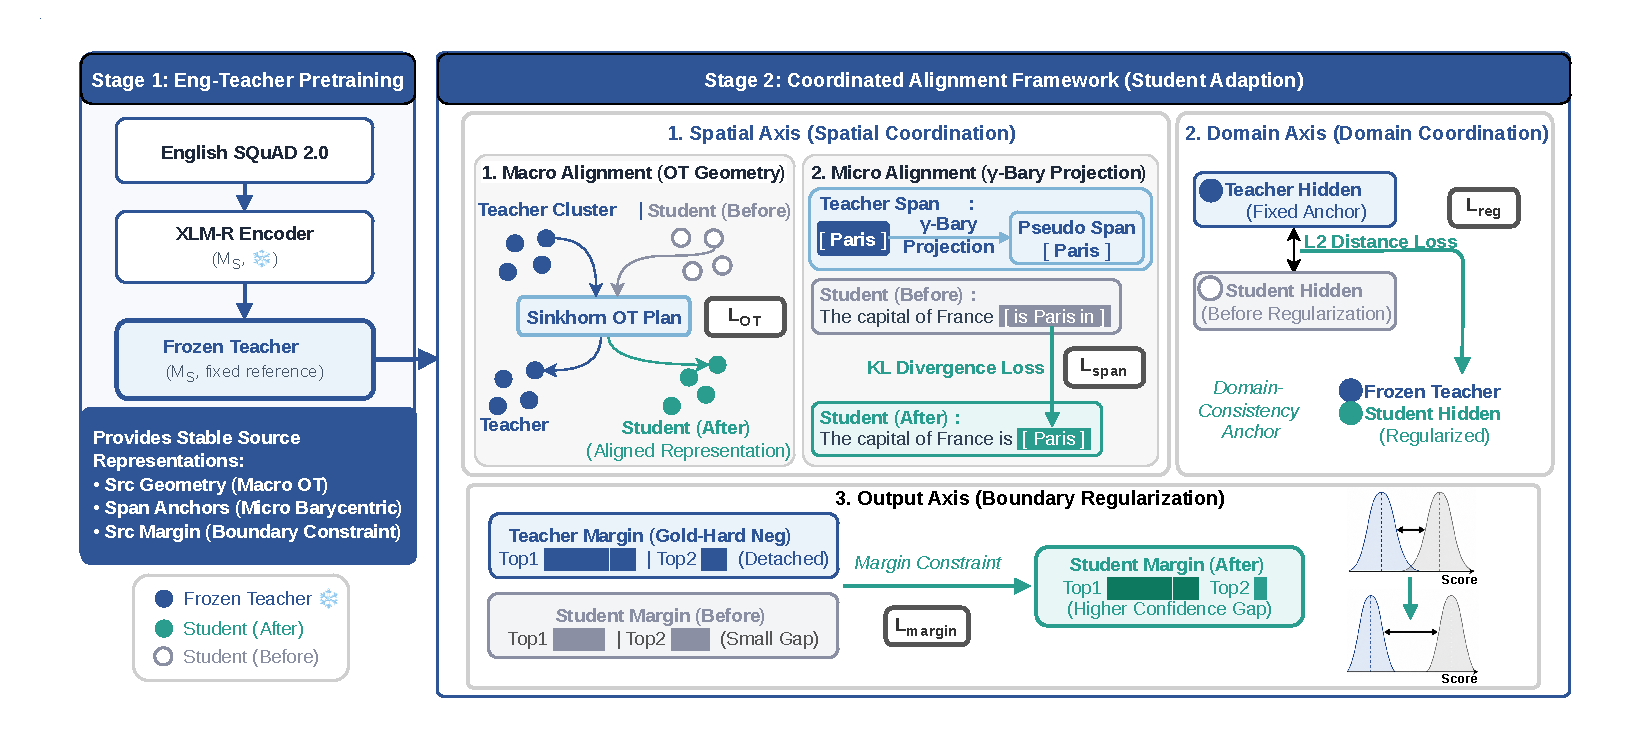
\includegraphics[width= 1.10\textwidth]{figures/main_framework.pdf}
    \caption{Overview of the proposed framework.}
    \label{fig:overview}
\end{figure*}


\subsection{Problem Formulation and Framework Overview}
To address the complementary failure modes of zero-shot cross-lingual transfer, we formulate the adaptation process as a coordinated optimization problem. Let $\mathcal{L}_{qa}$ denote the standard supervised question answering loss on the source language. We propose a framework whose core mechanism jointly coordinates spatial alignment and domain (source-language) preservation, plus a boundary-regularization term whose scheduling we study empirically in Section~\ref{sec:margin_impact}:
$$ \min_\theta \mathcal{L}_{total} = \lambda_{qa}\mathcal{L}_{qa} + \mathcal{L}_{space} + \mathcal{L}_{domain} + \mathcal{L}_{time} $$

We adopt a two-stage training paradigm utilizing a Teacher-Student architecture. In Stage 1, a teacher model is fine-tuned on the source language (English) to establish highly discriminative QA boundaries. In Stage 2, we freeze the teacher's weights and introduce a Low-Rank Adaptation (LoRA) student. 

Rather than relying solely on the final transformer layer -- which over-fits to task-specific predictive patterns -- we apply a trainable softmax weighting across intermediate layers 6--9 to extract language-agnostic semantic abstractions, since these layers are known to capture core structural and syntactic relations such as dependency syntax and coreference \citep{clark-etal-2019-bert}. The student is then optimized under spatial and domain coordination over these aggregated representations, with boundary regularization applied on top.

\subsection{Spatial Coordination: Macro and Micro Alignment}
\label{sec:spatial}
The spatial dimension ($\mathcal{L}_{space}$) aims to bridge the cross-lingual representation gap. We decompose this into macro-structural alignment via Optimal Transport ($\mathcal{L}_{ot}$) and micro-structural label projection via barycentric mapping ($\mathcal{L}_{span}$).

\textbf{Macro Alignment (OT):} Let $H^{src}$ and $H^{tgt}$ denote the normalized hidden representations of the source and target sequences at the intermediate layers. We define the transport cost matrix $C$ using the cosine distance:
$$ C_{ij} = 1 - \frac{h^{src}_i \cdot h^{tgt}_j}{\|h^{src}_i\| \|h^{tgt}_j\|} $$
We utilize the entropy-regularized Sinkhorn algorithm to find the optimal transport plan $T^*$. Crucially, we stop the gradient through the transport plan ($T^*.detach()$) so that the optimization only updates the representation geometry while treating the transport assignment as a fixed correspondence:
$$ \mathcal{L}_{ot} = \langle T^*.detach(), C \rangle_F $$
Minimizing $\mathcal{L}_{ot}$ in isolation pulls every target token toward a source-side barycenter defined by its transport-plan column; Appendix~\ref{sec:appendix_ot_theory} gives a first-order local argument that this can contract the representations of distinct target tokens whose matched-source neighborhoods overlap -- exactly the adjacent-token situation that answer-boundary detection must resolve -- which is why $\mathcal{L}_{ot}$ alone is insufficient and must be coordinated with the micro-alignment and boundary-regularization terms below.

\textbf{Micro Alignment ($\gamma$-Barycentric Span Transfer):} Extractive QA requires precise token-level boundary detection. Standard cross-lingual distillation minimizes the divergence between source and target logits, but this fails when vocabulary dimensions mismatch or span positions shift across translations. To solve this, we leverage the learned transport plan $\gamma$ (equivalent to $T^*$) to structurally project the source model's predicted span distribution ($p^{src}$) into the target space, creating zero-shot pseudo-labels ($\tilde{p}^{tgt}$):
$$ \tilde{p}^{tgt}_{start} = \frac{\gamma^T p^{src}_{start}}{\sum_i \gamma_{ij}} $$
The span-aware local alignment is then enforced via Kullback-Leibler divergence:
$$ \mathcal{L}_{span} = \frac{1}{2} \sum_{k \in \{start, end\}} D_{KL}(\tilde{p}^{tgt}_{k} \| p^{tgt}_{k}) $$
The total spatial coordination loss is defined as: $\mathcal{L}_{space} = \lambda_{ot}\mathcal{L}_{ot} + \lambda_{span}\mathcal{L}_{span}$.

\subsection{Domain Coordination: Source Preservation}
\label{sec:domain}
While spatial alignment successfully transfers semantic knowledge, updating shared parameters inherently risks corrupting well-established source language representations. To mitigate catastrophic forgetting, we coordinate the source domain ($\mathcal{L}_{domain}$).

Standard practices typically employ either strict parameter freezing (which heavily restricts cross-lingual adaptation capacity) or joint fine-tuning (which is computationally expensive and prone to gradient interference). Instead, we introduce a soft constraint mechanism. We minimize the $L_2$ distance between the token representations generated by the frozen English teacher ($h^{frz}_{src}$) and the actively adapting LoRA student ($h^{LoRA}_{src}$):
\[
\begin{aligned}
\mathcal{L}_{domain} &= \lambda_{reg}\mathcal{L}_{reg}, \\
\mathcal{L}_{reg} &= \frac{1}{|\mathcal{T}|}
\sum_{i \in \mathcal{T}}
\left\|h^{LoRA}_{src,i} - h^{frz}_{src,i}\right\|^2_2.
\end{aligned}
\]
This highly weighted regularization acts as a robust domain-consistency anchor, ensuring the student network safely adapts to the target language without drifting from the source model's structural topology.

\subsection{Boundary Regularization}
\label{sec:temporal}
Beyond spatial and domain coordination, we hypothesized that pulling target representations towards the source space all at once might blur the precise inter-token distinctions required for exact span extraction, and that protecting these boundaries would require a margin constraint directly in the task decision boundary (logit space). We test this hypothesis, and in particular whether the schedule of this constraint over training matters, empirically in Section~\ref{sec:margin_impact}.

We define the source margin ($m_{src}$) as the confidence gap between the gold token logit and the hardest negative token logit, while the target margin ($m_{tgt}$) is the difference between its top-1 and top-2 logits:
$$ m_{src} = \max\Big(0, \text{logit}[s^{gold}] - \max_{j \neq gold} \text{logit}[j]\Big) $$
$$ m_{tgt} = \text{top1\_logit} - \text{top2\_logit} $$
$$ \mathcal{L}_{margin} = \text{ReLU}(m_{src}.detach() - m_{tgt}) $$

We clamp $m_{src}$ at zero since a negative value only signals a teacher
misranking, not a genuine boundary target worth propagating. We compare two strategies for weighting this constraint over training: a \emph{static} strategy that holds the coefficient constant ($m=1.0$ throughout), and a \emph{dynamic} strategy that anneals it in discrete steps ($1.0 \rightarrow 0.7 \rightarrow 0.5 \rightarrow 0.3$ across 6 epochs). The complete static and dynamic schedules are shown in Appendix~\ref{sec:appendix_implementation} (Figure~\ref{fig:margin_schedule}). We hypothesized dynamic scheduling would outperform static by first anchoring boundaries strictly, then relaxing to let target-language representations settle; Section~\ref{sec:margin_impact} tests this with multi-seed evaluation and finds it \emph{not} supported. We denote the (possibly time-dependent) coefficient $m(\epsilon)$ scaling the margin loss as $\mathcal{L}_{time} = m(\epsilon)\,\mathcal{L}_{margin}$; the peak value $\lambda_{margin}=1.0$ in Table~\ref{tab:hyperparameters} is the constant used by the static strategy and the epoch-1 value of the dynamic schedule (see Appendix~\ref{sec:appendix_sensitivity} for how this differs from the fixed $\lambda_{ot}, \lambda_{span}, \lambda_{reg}$).



\subsection{Overall Objective}
By integrating the aforementioned components, our coordinated alignment framework combines spatial transfer and domain consistency as its core mechanism, with boundary regularization applied on top:
$$ \mathcal{L}_{total} = \lambda_{qa}\mathcal{L}_{qa} + \mathcal{L}_{space} + \mathcal{L}_{domain} + \mathcal{L}_{time} $$

\section{Experiments}
\label{sec:setup}

\textbf{Datasets and Evaluation:} We validate our coordinated alignment framework on extractive QA. In Stage 1, the teacher model is fine-tuned on the English SQuAD 2.0 dataset \citep{rajpurkar-etal-2018-know}. For Stage 2 (student adaptation), we utilize a parallel loader containing English SQuAD 2.0 and the AIForge Vietnamese-SQuAD dataset. Crucially, while the model sees unlabeled Vietnamese question/context text through this parallel loader, the student never receives target-language ground-truth answer labels during training; we refer to this as a \emph{target-label-free} cross-lingual transfer paradigm, distinct from a fully blind protocol in which the target language is never observed in any form. Following convention in this literature \citep{artetxe-etal-2020-cross, pfeiffer-etal-2020-mad}, \emph{zero-shot} here denotes the absence of target-language training labels, not of any target-language signal; our checkpoint selection does use target-language validation performance, which we discuss and stress-test in the Limitations section. We evaluate the transfer performance on the Vietnamese splits of XQuAD \citep{artetxe-etal-2020-cross} and MLQA \citep{lewis-etal-2020-mlqa}. 

\textbf{Metrics:} We report the standard Exact Match (EM) and macro-averaged F1 scores. To explicitly measure the catastrophic forgetting of the source language, we introduce the Source Preservation Metric ($\Delta_{src}$), defined as the difference in English SQuAD 2.0 F1 scores before and after the Stage-2 student alignment ($\Delta_{src} = F1_{post-align} - F1_{pre-align}$). An optimal framework should maximize target-language EM/F1 while maintaining $\Delta_{src} \approx 0$.

\textbf{Scope of Comparison:} Our primary evaluation compares our framework against the zero-shot XLM-R baseline, Vanilla KD, and controlled ablations (Table~\ref{tab:main_results}). We additionally evaluate adapter-based transfer (MAD-X-style), sentence-level contrastive alignment (InfoXLM-inspired), and global OT posterior alignment (MINOTAUR-inspired), all retrained end-to-end under our exact protocol on all three target languages. These three are task-adapted implementations of the core mechanism proposed in each cited work -- adapted to our SQuAD-2.0/answerability setting and retrained under our own protocol -- rather than reproductions of the original papers' full training recipes; we retain the short names (MAD-X, InfoXLM, MINOTAUR) in tables for brevity. Implementation details, retraining protocol, and full cross-language discussion for all four baselines are provided in Appendix~\ref{sec:appendix_baselines}.

\textbf{Implementation Details:} Our framework is built upon the XLM-RoBERTa backbone \citep{conneau-etal-2020-unsupervised}. For parameter-efficient training in Stage 2, we apply Low-Rank Adaptation (LoRA) \citep{hu2021loralowrankadaptationlarge} to the query, key, value, and dense projection matrices with rank $r=16$ and $\alpha=32$. The dynamic margin schedule anneals the threshold in discrete temporal steps (from $1.0$ down to $0.3$) across the training epochs. 

\subsection{Main Results: Zero-Shot Cross-Lingual Transfer}

Table~\ref{tab:main_results} summarizes zero-shot transfer performance across Vietnamese, Arabic, and Hindi. Our coordinated framework consistently improves XQuAD over the zero-shot baseline in all three languages while maintaining competitive MLQA performance, where gains are generally smaller. Vanilla KD remains nearly identical to the zero-shot baseline, indicating that logit-level distillation alone provides little transfer benefit. All retrained external baselines (MAD-X, InfoXLM, and MINOTAUR) underperform both the zero-shot baseline and our method, suggesting that adapter transfer, sentence-level contrastive alignment, and global-only OT posterior alignment are each insufficient for robust cross-lingual QA on their own.

The same qualitative trend holds for Arabic and Hindi. Across both languages, our framework consistently improves XQuAD while preserving competitive MLQA performance, whereas Vanilla KD remains close to the zero-shot baseline and all external baselines underperform. Table~\ref{tab:main_results} reports single-run (seed 42) comparisons for strict consistency with the ablation study; multi-seed evaluation of our own framework (Section~\ref{sec:margin_impact}; Appendix~\ref{sec:appendix_ar_hi_multiseed}) confirms that Ours' target-language gains are stable rather than seed-specific. The external baselines (Vanilla KD, MAD-X, InfoXLM, MINOTAUR) are evaluated at a single seed only, so we do not claim their relative ranking is seed-robust. Detailed per-language analysis is provided in Appendix~\ref{sec:appendix_baselines}.
\begin{table*}[t]
\centering
\begin{tabular}{llcccc}
\toprule
\multirow{2}{*}{\textbf{Target Language}} & \multirow{2}{*}{\textbf{Model}} & \multicolumn{2}{c}{\textbf{XQuAD}} & \multicolumn{2}{c}{\textbf{MLQA}} \\
\cmidrule(lr){3-4} \cmidrule(lr){5-6}
 & & \textbf{EM} & \textbf{F1} & \textbf{EM} & \textbf{F1} \\
\midrule
\multirow{6}{*}{Vietnamese}
 & XLM-R Zero-shot & 46.22 & 63.64 & 46.05 & 67.21 \\
 & Vanilla KD \citep{hinton2015distillingknowledgeneuralnetwork} & 46.97 & 63.58 & \textbf{46.10} & 67.21 \\
 & MAD-X \citep{pfeiffer-etal-2020-mad} & 42.69 & 57.03 & 34.85 & 48.52 \\
 & InfoXLM \citep{chi-etal-2021-infoxlm} & 28.49 & 38.29 & 43.24 & 64.48 \\
 & MINOTAUR \citep{sherborne-etal-2023-optimal} & 41.26 & 58.05 & 41.42 & 61.79 \\
 & \textbf{Ours (Coordinated, static)} & \textbf{49.70} & \textbf{69.73} & 46.00 & \textbf{67.60} \\
\midrule
\multirow{6}{*}{Arabic}
 & XLM-R Zero-shot & 43.53 & 57.03 & 37.26 & 56.38 \\
 & Vanilla KD \citep{hinton2015distillingknowledgeneuralnetwork} & 43.95 & 57.13 & 37.22 & 56.12 \\
 & MAD-X \citep{pfeiffer-etal-2020-mad} & 32.35 & 45.79 & 21.44 & 33.89 \\
 & InfoXLM \citep{chi-etal-2021-infoxlm} & 23.45 & 30.96 & 34.47 & 53.71 \\
 & MINOTAUR \citep{sherborne-etal-2023-optimal} & 36.72 & 50.04 & 33.54 & 52.81 \\
 & \textbf{Ours (Coordinated, static)} & \textbf{47.31} & \textbf{65.26} & \textbf{37.59} & \textbf{56.5} \\
\midrule
\multirow{6}{*}{Hindi}
 & XLM-R Zero-shot & 44.54 & 60.21 & 42.88 & 60.4 \\
 & Vanilla KD \citep{hinton2015distillingknowledgeneuralnetwork} & 44.79 & 60.37 & 42.80 & 60.41 \\
 & MAD-X \citep{pfeiffer-etal-2020-mad} & 42.52 & 52.84 & 33.75 & 43.98 \\
 & InfoXLM \citep{chi-etal-2021-infoxlm} & 35.38 & 47.04 & 41.46 & 59.62 \\
 & MINOTAUR \citep{sherborne-etal-2023-optimal} & 29.75 & 42.78 & 36.93 & 53.41 \\
 & \textbf{Ours (Coordinated, static)} & \textbf{52.94} & \textbf{66.94} & \textbf{45.87} & \textbf{61.69} \\
\bottomrule
\end{tabular}
\caption{Zero-shot cross-lingual QA results on XQuAD and MLQA (seed 42). Multi-seed validation of our framework is reported in Section~\ref{sec:margin_impact} (Vietnamese) and Appendix~\ref{sec:appendix_ar_hi_multiseed} (Arabic/Hindi). External baselines are single-seed; see Appendix~\ref{sec:appendix_baselines}.}
\label{tab:main_results}
\end{table*}

\subsection{Source Preservation Analysis}
A critical failure mode in cross-lingual adaptation is the degradation of source-language capabilities from shared parameter updates: frameworks employing global spatial alignment without domain constraints suffer severe catastrophic forgetting, evidenced by a significant drop in English QA performance ($\Delta_{src} \ll 0$). 

By integrating the domain-consistency anchor ($\mathcal{L}_{reg}$), our domain coordination mechanism successfully restricts the LoRA parameters from unlearning English syntax. The student model maintains a $\Delta_{src}$ approximating zero, providing empirical evidence that target-language topological mapping can be achieved without paying a substantial alignment tax on the source language.

Table~\ref{tab:source_preservation} evaluates source-language preservation after Stage-2 adaptation. Vanilla KD leaves English performance essentially unchanged across all benchmarks and all three target languages ($\Delta_{src}$ within $\pm0.16$ on in-domain SQuAD-EN), confirming that distillation alone introduces little interference with the shared encoder -- but Table~\ref{tab:main_results} shows this comes at the cost of essentially no target-language transfer. In contrast, MINOTAUR, which employs global OT without domain coordination, suffers severe catastrophic forgetting, particularly on held-out English benchmarks. Our framework keeps $\Delta_{src}$ close to zero (within roughly $\pm1.2$ F1 across SQuAD-EN, XQuAD-en, and MLQA-en) while delivering the largest target-language gains of any method evaluated (Table~\ref{tab:main_results}): Ours provides the best transfer--retention trade-off, while Vanilla KD preserves English marginally more tightly but produces little target-language improvement.
The same qualitative pattern holds across the other retrained baselines: MAD-X, InfoXLM, and MINOTAUR all show larger source-side degradation than either Vanilla KD or our framework, without matching our framework's target-language gains. Detailed per-baseline analyses are provided in Appendix~\ref{sec:appendix_baselines}.
\begin{table*}[t]
\centering
\small
\resizebox{\textwidth}{!}{%
\begin{tabular}{lcccccccccc}
\toprule
\multirow{2}{*}{\textbf{Configuration}} & \multicolumn{3}{c}{\textbf{SQuAD-EN (in-domain)}} & \multicolumn{3}{c}{\textbf{XQuAD-en (held-out)}} & \multicolumn{3}{c}{\textbf{MLQA-en (held-out)}} \\
\cmidrule(lr){2-4} \cmidrule(lr){5-7} \cmidrule(lr){8-10}
 & \textbf{Pre F1} & \textbf{Post F1} & \textbf{$\Delta_{src}$} & \textbf{Pre F1} & \textbf{Post F1} & \textbf{$\Delta_{src}$} & \textbf{Pre F1} & \textbf{Post F1} & \textbf{$\Delta_{src}$} \\
\midrule
Teacher (Stage 1 only) & 72.84 & 72.84 & 0.0 & 75.7 & 75.7 & 0.0 & 79.8 & 79.8 & 0.0 \\
\midrule
\multicolumn{10}{l}{\textbf{Vietnamese}} \\
Vanilla KD & 72.84 & 73.00 & 0.16 & 75.7 & 76.34 & 0.64 & 79.8 & 79.80 & 0.00 \\
MAD-X & 72.84 & 78.21 & 5.37 & 75.7 & 74.82 & -0.88 & 79.8 & 62.05 & -17.75 \\
InfoXLM & 72.84 & 70.35 & -2.49 & 75.7 & 59.10 & -16.60 & 79.8 & 78.47 & -1.33 \\
MINOTAUR & 72.84 & 64.09 & -8.75 & 75.7 & 56.32 & -19.38 & 79.8 & 77.31 & -2.49 \\
Ours & 72.84 & 74.02 & 1.18 & 75.7 & 74.78 & -0.92 & 79.8 & 79.5 & -0.3 \\
\midrule
\multicolumn{10}{l}{\textbf{Arabic}} \\
Vanilla KD & 72.84 & 72.90 & 0.06 & 75.7 & 76.63 & 0.93 & 79.8 & 79.85 & 0.05 \\
MAD-X & 72.84 & 78.21 & 5.37 & 75.7 & 74.82 & -0.88 & 79.8 & 62.05 & -17.75 \\
InfoXLM & 72.84 & 69.32 & -3.52 & 75.7 & 59.06 & -16.64 & 79.8 & 76.82 & -2.98 \\
MINOTAUR & 72.84 & 61.32 & -11.52 & 75.7 & 51.49 & -24.21 & 79.8 & 76.36 & -3.44 \\
Ours & 72.84 & 72.57 & -0.27 & 75.7 & 76.81 & 1.11 & 79.8 & 79.52 & -0.28 \\
\midrule
\multicolumn{10}{l}{\textbf{Hindi}} \\
Vanilla KD & 72.84 & 72.83 & -0.01 & 75.7 & 76.45 & 0.75 & 79.8 & 79.90 & 0.10 \\
MAD-X & 72.84 & 78.21 & 5.37 & 75.7 & 74.82 & -0.88 & 79.8 & 62.05 & -17.75 \\
InfoXLM & 72.84 & 71.51 & -1.33 & 75.7 & 64.07 & -11.63 & 79.8 & 78.48 & -1.32 \\
MINOTAUR & 72.84 & 61.61 & -11.23 & 75.7 & 44.08 & -31.62 & 79.8 & 77.59 & -2.21 \\
Ours & 72.84 & 72.66 & -0.18 & 75.7 & 76.87 & 1.17 & 79.8 & 79.86 & 0.06 \\
\bottomrule
\end{tabular}
}
\caption{Analysis of source preservation ($\Delta_{src}$) on English SQuAD 2.0 (in-domain, i.e.\ the Stage-1 training distribution), alongside held-out English XQuAD-en and MLQA-en on single seed 42 (the exact English counterparts of the cross-lingual transfer targets used elsewhere in this paper). Multi-seed validation for the selected static margin configuration is detailed in Appendix~\ref{sec:appendix_vi_multiseed} (for Vietnamese) and Appendix~\ref{sec:appendix_ar_hi_multiseed} (for Arabic and Hindi). $\Delta_{src} = F1_{post\text{-}align} - F1_{pre\text{-}align}$. The external baselines described in Appendix~\ref{sec:appendix_baselines}.}
\label{tab:source_preservation}
\end{table*}

\subsection{Ablation Study}
\label{sec:ablation_study}
To isolate the contributions of the spatial and temporal coordination mechanisms, we conduct an extensive ablation study (Table~\ref{tab:ablation_study}); a full discussion of external baselines, including Vanilla KD, is instead given in Appendix~\ref{sec:appendix_baselines}. Every configuration M2--M5 retains the domain-consistency term ($\mathcal{L}_{reg}$); its individual contribution is isolated in Table~\ref{tab:source_preservation}, where MINOTAUR -- an external published method that, unlike M2, performs unregulated cross-lingual alignment \emph{without} any domain-consistency anchor, via a distributionally different mechanism than M2's token-level transport plan (sentence-level Gaussian posterior alignment; Appendix~\ref{sec:appendix_minotaur}) -- leaves in-domain SQuAD-EN measurably degraded and held-out English F1 far more severely damaged (Vietnamese XQuAD-en $\Delta_{src}=-19.38$) relative to the pre-alignment teacher, consistent with catastrophic forgetting that widens on held-out rather than in-domain data.

\begin{table}[t]
\centering
\small
\resizebox{\columnwidth}{!}{%
\begin{tabular}{lccccc}
\toprule
 & \textbf{M1} & \textbf{M2} & \textbf{M3} & \textbf{M4} & \textbf{M5 (Ours)} \\
\midrule
Global ($\mathcal{L}_{ot}$) & $\times$ & $\checkmark$ & $\checkmark$ & $\checkmark$ & $\checkmark$ \\
Local ($\mathcal{L}_{span}$) & $\times$ & $\times$ & $\checkmark$ & $\checkmark$ & $\checkmark$ \\
Time ($m$) & $\times$ & $\times$ & $\times$ & Dyn. & Static \\
\midrule
MLQA-vi EM & \textbf{46.05} & 42.89 & 44.35 & 45.23 & 46 \\
MLQA-vi F1 & 67.21 & 64.08 & 65.33 & 67.33 & \textbf{67.6} \\
SQuAD-EN EM & 64.26 & 65.63 & 64.58 & \textbf{66.21} & 65.69 \\
SQuAD-EN F1 & 72.84 & 73.89 & 73.09 & \textbf{74.37} & 74.02 \\
\bottomrule
\end{tabular}
}
\caption{Ablation study of the coordinated alignment framework (single seed, epoch-3 checkpoint; see Table~\ref{tab:heldout_source} for the multi-seed M4--M5 comparison). M1 is the zero-shot baseline; M2--M5 progressively add global alignment ($\mathcal{L}_{ot}$), span projection ($\mathcal{L}_{span}$), and boundary regularization ($m$, dynamic in M4, static in M5), while retaining domain consistency ($\mathcal{L}_{reg}$). External baselines are reported separately (Table~\ref{tab:main_results}, Appendix~\ref{sec:appendix_baselines}). M5 (static) is the recommended default based on the multi-seed evaluation in Section~\ref{sec:margin_impact}.}
\label{tab:ablation_study}
\end{table}

Configuration M2 ($\mathcal{L}_{ot}$ plus the domain-consistency anchor, without span-aware or boundary regularization) measurably reduces overall F1 relative to the zero-shot baseline M1, showing that global-only spatial alignment can still hurt transfer even with the domain-consistency anchor active -- though Appendix~\ref{sec:appendix_reg_ablation} shows the decline is real but moderate rather than severe (this pattern replicates on Arabic and Hindi as well, Appendix~\ref{sec:appendix_arabic_hindi_margin}). Adding the micro-alignment term (M3, $\mathcal{L}_{span}$) largely recovers this loss and improves Exact Match, confirming that span-aware local alignment is necessary to convert global transport into precise boundary localization. Boundary regularization (M4, M5) then yields further, consistent target-side gains over M3, while source-side performance (SQuAD-EN) stays within a narrow band (73.09--74.37 F1) since $\mathcal{L}_{reg}$ is active throughout; M4 vs.\ M5 makes little difference at this single-seed checkpoint, with the full multi-seed comparison in Section~\ref{sec:margin_impact}. Every configuration in Table~\ref{tab:ablation_study} keeps $\mathcal{L}_{reg}$ active, so it does not by itself isolate the anchor's marginal contribution; Appendix~\ref{sec:appendix_reg_ablation} reports a single-seed exploratory comparison against a matched configuration with $\mathcal{L}_{reg}$ removed, finding the anchor gives a modest, broadly consistent benefit across most benchmarks, though we still treat this as suggestive rather than conclusive given the single seed.

\subsection{Does Boundary Regularization Need to Be Dynamically Scheduled? A Multi-Seed Test}
\label{sec:margin_impact}

Section~\ref{sec:temporal} motivated a dynamic schedule for the boundary-regularization coefficient $m(\epsilon)$. We test this hypothesis directly by contrasting the dynamic schedule (M4) against the static strategy (M5, constant $m=1.0$) across three random seeds (42, 43, 44) on every benchmark. Training trajectories and detailed tabular results for the dynamic and static strategies are provided in Appendix~\ref{sec:appendix_vi_multiseed}.

The results do not support our original hypothesis. On the two target-language benchmarks that matter most for this paper's central claim, the static strategy is reliably better: on XQuAD-vi, the paired difference favors M5 on both EM and F1 across all 3 seeds (with a mean paired advantage of $+0.68$ EM and $+0.86$ F1). On MLQA-vi, M5 is consistently ahead on EM across all 3 seeds, while the two are near-indistinguishable on F1. On the source side, the pattern is mixed: M4 has a consistent edge on the in-domain SQuAD-EN benchmark, while M5 is consistently ahead on the held-out XQuAD-en benchmark. 

We report this as a negative result rather than reframing it post-hoc: a boundary-regularization term's presence clearly matters (Section~\ref{sec:ablation_study} shows M3 without a margin term underperforms), but \emph{how} that term is scheduled over training does not reliably matter here. We recommend the static strategy (M5) as the default: it is simpler (no schedule to tune) and at least as good, measurably better on our primary target metric. This finding is further corroborated by matched multi-seed comparisons on Arabic (Appendix~\ref{sec:appendix_arabic_hindi_margin}), which also directionally favor static scheduling on the target side.

\section{Conclusions}
In this paper, we demonstrated that the persistent trade-off between cross-lingual transfer and source-language retention in zero-shot extractive QA stems from uncoordinated optimization. We show this concretely: global-only spatial alignment -- OT without span-aware local projection or boundary regularization -- can underperform a zero-shot baseline, replicated across three target languages.

To resolve this, we proposed a framework that coordinates spatial alignment with a domain-consistency anchor protecting source-language representations, recovering and exceeding zero-shot performance where global-only spatial alignment fails. We additionally introduced a margin-based boundary-regularization term and tested, via multi-seed evaluation, whether it should be scheduled dynamically over training. We found no reliable evidence that it should: a constant constraint is at least as effective, and on our primary Vietnamese target benchmark, measurably more consistent. We report this negative result in full, since it clarifies that boundary
regularization's value lies in its presence rather than its schedule. Empirical evaluations confirm that the resulting coordinated framework enhances zero-shot cross-lingual transfer while largely maintaining source-language reading comprehension across both in-domain and held-out benchmarks.

\section*{Limitations}
While our coordinated alignment framework provides a robust solution for cross-lingual transfer, we acknowledge several limitations.

First, the spatial coordination relies on the entropy-regularized Sinkhorn algorithm, which computes a dense cost matrix ($\mathcal{O}(L^2)$). Although manageable for standard QA contexts via dynamic truncation, it introduces a 3.8$\times$ wall-clock slowdown (Appendix~\ref{sec:appendix_complexity}) and memory overhead for long contexts. Future work may explore linear-time OT approximations or Sliced Wasserstein Distances.

Second, although the framework is target-label-free (no target-language QA annotations are required), the OT cost matrix still depends on parallel bilingual corpora. This restricts immediate applicability to fully unsupervised, monolingual-only settings.

Third, our deep analysis focuses primarily on English–Vietnamese, enabling extensive ablations and multi-seed evaluation within computational constraints. Multi-seed results on Arabic and Hindi confirm the core benefit (Appendix~\ref{sec:appendix_ar_hi_multiseed}), but also reveal language-specific dynamics (e.g., weaker margin-schedule effects for Arabic and early-epoch instability for Hindi). Broader typological coverage remains important future work.

Fourth, our checkpoint selection is target-informed rather than fully blind. A fixed stopping point yields comparable results on Vietnamese and Arabic, though Hindi relies more on early stopping (Appendix~\ref{sec:appendix_hindi_anomaly}). A purely source-based selection criterion is left for future work. In addition, while Table~\ref{tab:ablation_study} isolates $\mathcal{L}_{span}$ and boundary regularization, every configuration retains $\mathcal{L}_{reg}$; a controlled multi-seed ablation isolating the domain-consistency anchor alone is also left for future work.


% Bibliography entries for the entire Anthology, followed by custom entries
%\bibliography{custom,anthology-overleaf-1,anthology-overleaf-2}

% Custom bibliography entries only
\bibliography{custom}

\appendix

\section{Theoretical Note: Why Unregularized Global OT Can Degrade Boundary Discriminability}
\label{sec:appendix_ot_theory}

Section~\ref{sec:ablation_study} shows empirically that global-only spatial alignment (configuration M2) underperforms the zero-shot baseline M1. Here we give a local, first-order argument for \emph{why} this is an expected consequence of the $\mathcal{L}_{ot}$ objective defined in Section~\ref{sec:spatial} rather than an incidental artifact of our particular setup. The argument isolates the single-step effect of the OT gradient on pairwise distances between target-token representations and connects that effect to the (near-)linear span-prediction head; it is not a full nonlinear convergence proof of training dynamics, and we state this scope limitation explicitly at the end.

\textbf{Setup.} All representations are $\ell_2$-normalized. Let $u_i = h_i^{src}/\|h_i^{src}\|$ and $v_j = h_j^{tgt}/\|h_j^{tgt}\|$. Since the gradient is stopped through the transport plan ($T^*.detach()$), $T^*$ is treated as a fixed coupling for the purpose of this analysis. (Note that on the unit sphere the cosine cost $C_{ij}=1-u_i^\top v_j$ coincides with the squared Euclidean cost $\frac12\|u_i-v_j\|^2$. We adopt the latter algebraic form solely for the local Euclidean analysis below; the two coincide numerically and the qualitative contraction pressure is identical after $\ell_2$-renormalization, which is how the loss is implemented in practice.)

\textbf{Local argument 1 (Barycentric pull direction).} A gradient-descent step on $\mathcal{L}_{ot} = \sum_{i,j} T^*_{ij}C_{ij}$ with respect to $v_j$ moves $v_j$ (prior to re-normalization) toward a barycenter. Using the Euclidean form $C_{ij} = \frac{1}{2}\|u_i - v_j\|^2$, the gradient is $\nabla_{v_j} C_{ij} = v_j - u_i$, so:
\begin{equation*}
-\nabla_{v_j}\mathcal{L}_{ot} = \sum_i T^*_{ij}\, (u_i - v_j) \;=\; m_j\,(\bar{u}_j - v_j),
\end{equation*}
where $m_j = \sum_i T^*_{ij}$ is the column mass and $\bar{u}_j = \frac{1}{m_j} \sum_i T^*_{ij} u_i$ is the weighted mean of the matched source directions. Thus, a gradient step pulls $v_j$ directly toward $\bar{u}_j$.

\textbf{Local argument 2 (Contraction of tokens with overlapping matches).} Consider two target tokens $p, q$ -- for instance, adjacent context positions that are both candidates for a span boundary. We assume the source tokens $\{u_i\}$ are sufficiently spread so that similar cost profiles imply similar transport columns. Because of the entropic regularization $\varepsilon > 0$, the Sinkhorn kernel $T^*_{ij} \propto \exp(-C_{ij}/\varepsilon)$ is Lipschitz in the cost with a constant proportional to $1/\varepsilon$. Whenever $v_p$ and $v_q$ start out close (an unavoidable situation for adjacent subwords sharing local context), the transport columns are close enough that their normalized barycenters satisfy $\|\bar{u}_p - \bar{u}_q\| \le \alpha$.

A gradient step $v_j^{(1)} = v_j - \eta \nabla_{v_j}\mathcal{L}_{ot} = (1-\eta m_j)v_j + \eta m_j \bar{u}_j$ (ignoring the subsequent $\ell_2$-renormalization for the local analysis) therefore moves $v_p$ and $v_q$ toward two attractor points that themselves lie within $\alpha$ of one another. Assuming similar local masses $m_p \approx m_q \approx m$ and absorbing $m$ into $\eta$:
\begin{equation*}
\|v_p^{(1)} - v_q^{(1)}\| \;\le\; (1-\eta)\,\|v_p-v_q\| + \eta\,\alpha.
\end{equation*}
As long as the transport plan remains approximately stable in a local neighborhood, repeated gradient steps drive the pairwise distance toward a value controlled by $\alpha$. Thus the local equilibrium distance between the two target representations is capped by the overlap of their matched-source neighborhoods ($\alpha$), \emph{regardless of their original separability} (whenever $\alpha$ is smaller than their initial distance). While subsequent $\ell_2$-renormalization slightly rescales Euclidean chord length, the angular contraction pressure remains. Since $\alpha$ grows with the entropy of the transport plan, this explains the diagnostic we track in Appendix~\ref{sec:appendix_hindi_anomaly} (Table~\ref{tab:hindi_entropy}), where higher-entropy plans coincide with the languages and epochs that exhibit the sharpest representational instability.

\textbf{Local argument 3 (Margin degradation).} The span-prediction head scores each candidate position via an approximately linear map $s(h)=w^\top h$, which is Lipschitz with constant $\|w\|$. For a correct boundary token $p$ and an adjacent distractor $q$ the achievable logit margin therefore satisfies
\begin{equation*}
\bigl|s(h_p)-s(h_q)\bigr| \le \|w\|\cdot d(h_p,h_q).
\end{equation*}
As Local argument~2 drives $d\to\alpha$, this margin is upper-bounded by $\|w\|\alpha$ irrespective of how well the task signal could otherwise separate $p$ from $q$. In other words, the $\mathcal{L}_{ot}$ gradient in isolation imposes a representation-level pressure toward a ceiling on answer-boundary precision -- a pressure that the span-aware and boundary-regularization terms below are specifically designed to counteract.

\textbf{Scope and caveats.} This is a local, first-order intuition rather than a proof of the full nonlinear training trajectory, and it assumes a locally Lipschitz span-prediction head. Critically, it isolates the gradient of $\mathcal{L}_{ot}$ alone; it is not a proof that configuration M2 as a whole (which also includes $\mathcal{L}_{qa}$ and the domain-consistency term $\mathcal{L}_{reg}$) must underperform M1 -- that is an empirical finding (Section~\ref{sec:ablation_study}), and this argument only supplies a plausibility mechanism for why the $\mathcal{L}_{ot}$ component of M2 pushes in that direction. It characterizes a contraction \emph{pressure} inherent to $\mathcal{L}_{ot}$, not a claim that the pressure is always realized to the degree the bound permits. $\mathcal{L}_{span}$ and $\mathcal{L}_{time}$ are deliberately designed to supply an opposing, boundary-preserving gradient (Sections~\ref{sec:spatial} and~\ref{sec:temporal}); the recovery of M3--M5 relative to M2 (Table~\ref{tab:ablation_study}) is consistent with this counteracting effect. We present the argument as a plausibility mechanism that explains, rather than merely redescribes, the pattern already visible in the M2 ablation and in the Sinkhorn-entropy diagnostics of Appendix~\ref{sec:appendix_hindi_anomaly}. Both phenomena are downstream symptoms of the same underlying OT pull, which is why we treat over-alignment granularity -- not either symptom in isolation -- as the shared root cause.

\section{Why Space and Domain Coordination Are Jointly Necessary}
\label{sec:appendix_three_axes}
We argue the space/domain coordination is not an arbitrary engineering choice but follows from the distinct level at which each operates: the spatial component addresses a \emph{representation-level} problem (where target tokens sit relative to source tokens in the shared embedding space), while the domain component addresses a \emph{parameter-level} problem (how much the shared encoder is permitted to drift while adapting). A failure at one level is not corrected by intervening at the other: Table~\ref{tab:ablation_study} illustrates this empirically. M2 already includes the domain-consistency anchor ($\mathcal{L}_{reg}$) alongside global-only spatial alignment ($\mathcal{L}_{ot}$), yet still degrades target-language transfer below the zero-shot baseline M1. This shows that domain coordination, while it protects source-language representations (SQuAD-EN F1 stays within a narrow 73.09--74.37 band across M2--M5 in Table~\ref{tab:ablation_study}), does not by itself correct the representation-level contraction on the target side that global-only spatial alignment induces (Appendix~\ref{sec:appendix_ot_theory}). Fixing that requires intervening at the same representation level, via the span-aware micro-alignment term ($\mathcal{L}_{span}$, M3) and boundary regularization (M4/M5) -- not via a further parameter-level constraint. This is the sense in which the two coordination mechanisms are jointly necessary: each addresses a failure mode the other cannot reach on its own.

We initially treated boundary regularization (Section~\ref{sec:temporal}) as a third, parallel axis operating at the optimization-schedule level. Our multi-seed evaluation (Section~\ref{sec:margin_impact}) complicates this picture: while the \emph{presence} of a boundary-regularization term clearly helps (M3, without any margin term, underperforms M4/M5 which include one), we find no reliable evidence that the term's specific \emph{schedule} over training is what matters -- a constant constraint performs as well as, and on our primary Vietnamese target benchmark, more consistently than, a dynamically annealed one. We therefore no longer present temporal scheduling as a coordinate axis on equal footing with space and domain; we instead treat it as a design choice within boundary regularization whose value we tested rather than assumed, and report the resulting negative result on scheduling specifically as one of this paper's contributions.

We do not claim the two-axis (space, domain) decomposition, plus a separately-evaluated boundary-regularization component, is the unique correct way to structure this problem -- a finer-grained scheme could, for instance, separate macro- and micro-alignment into distinct axes within space. But it is the coarsest partition at which each retained axis maps cleanly onto a distinct, empirically-confirmed failure mode (over-alignment and catastrophic forgetting, respectively), which is why we adopt it as the natural granularity for this problem.

\section{Implementation Details and Hyperparameters}
\label{sec:appendix_implementation}
To facilitate absolute reproducibility, we provide comprehensive specifications regarding our multi-stage architecture, optimization configurations, and data tokenization pipelines.

\begin{figure}[t]
    \centering
    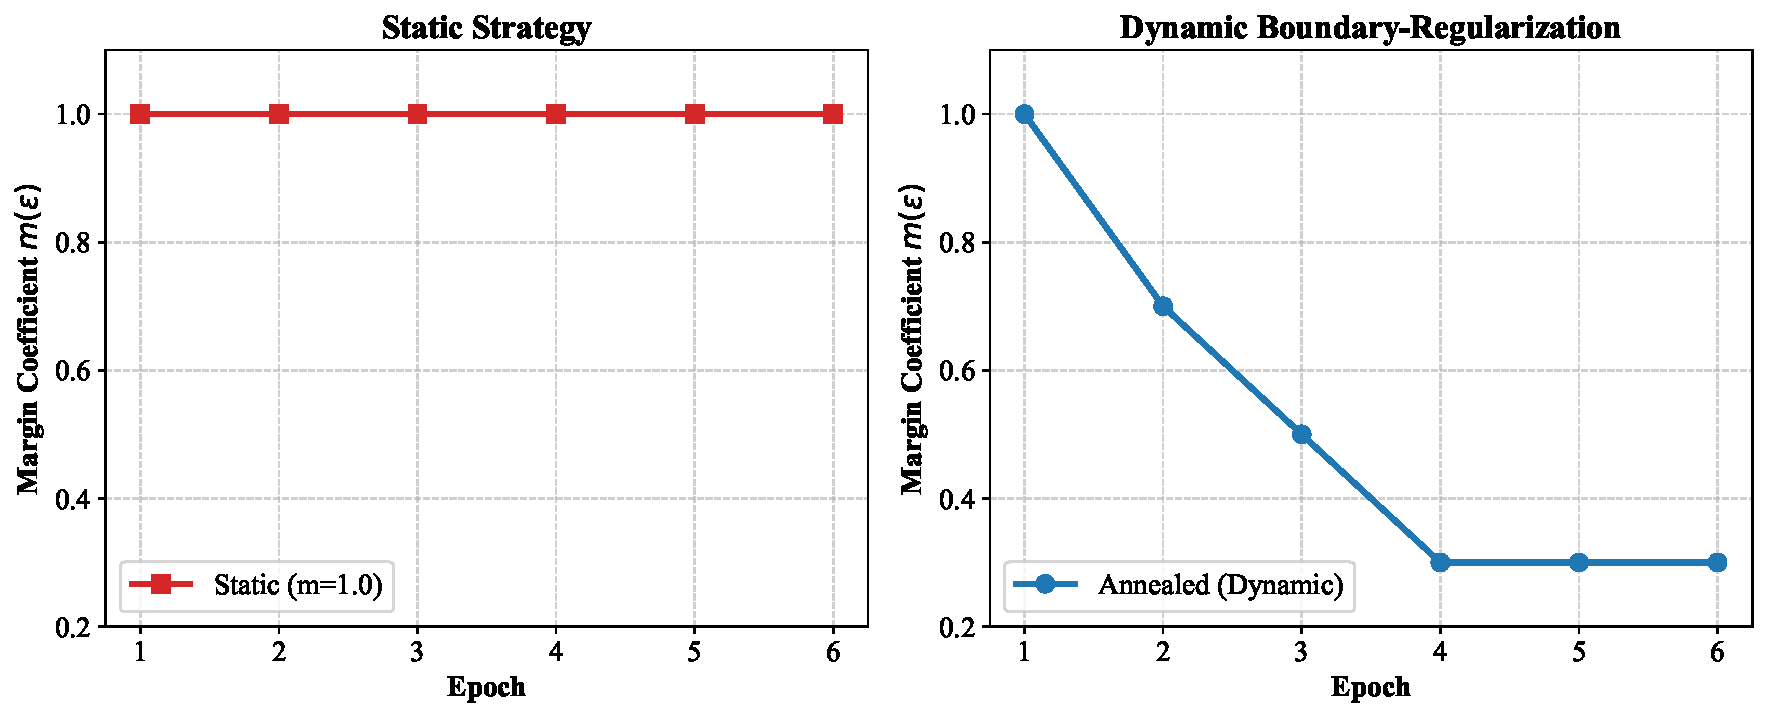
\includegraphics[width= 1\linewidth]{figures/margin_schedule.pdf}
    \caption{Static and dynamic boundary-regularization schedules evaluated in Section~\ref{sec:margin_impact}.}
    \label{fig:margin_schedule}
\end{figure}

\begin{figure*}[t]
    \centering
    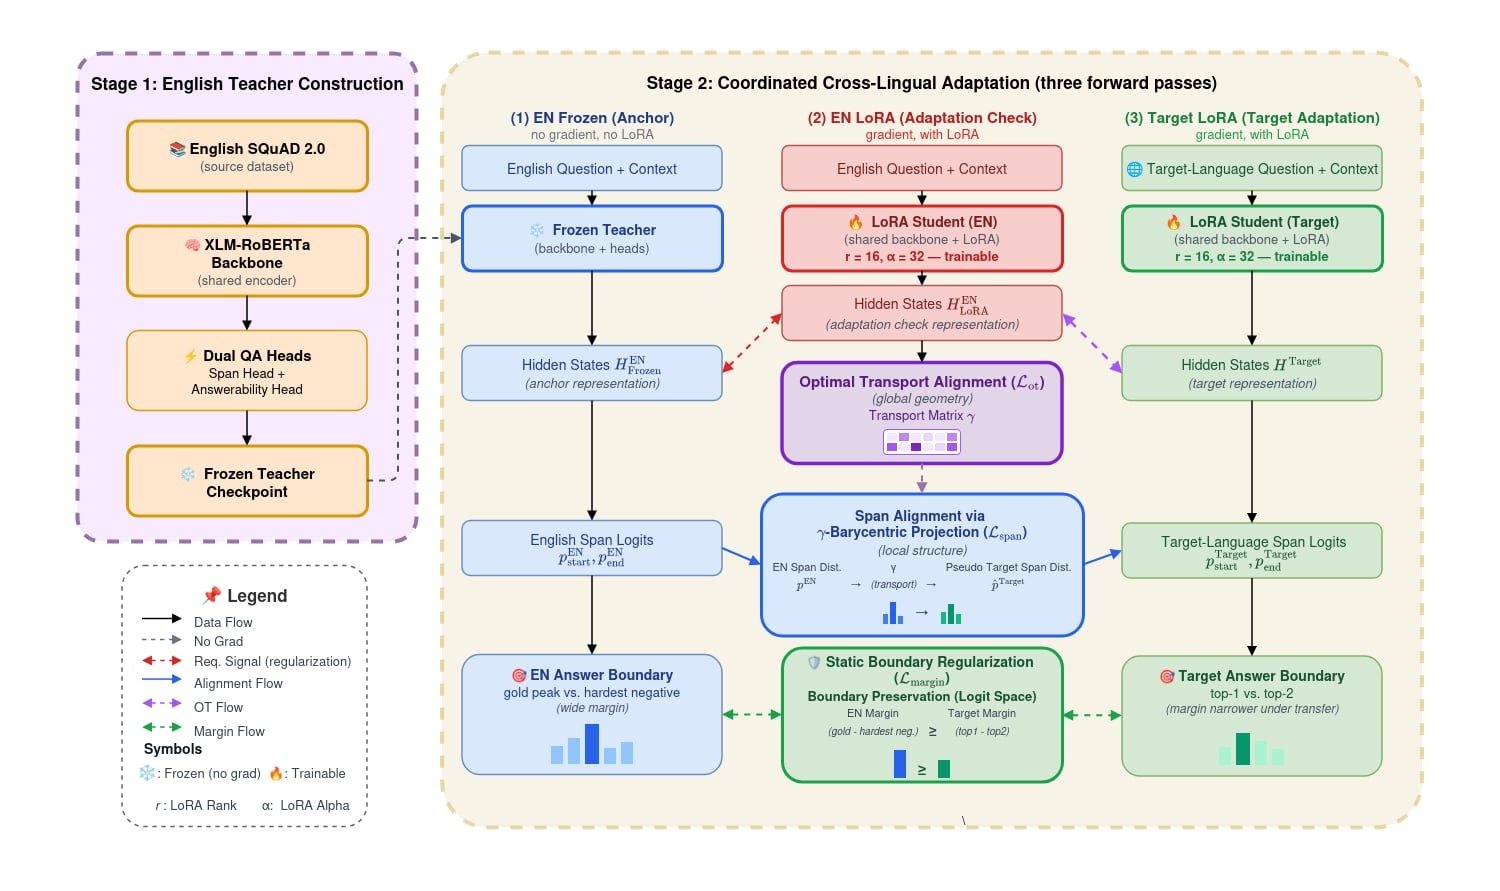
\includegraphics[width=\textwidth]{figures/pipeline.png}
    \caption{Overview of our Coordinated Alignment Framework. Rather than relying on a monolithic alignment objective, we decouple the cross-lingual transfer process into two core coordination axes -- Spatial Alignment, which resolves the representation gap via Optimal Transport plus span-aware local projection, and Source Preservation, which mitigates catastrophic forgetting via a domain-consistency anchor -- each addressing a failure mode the other cannot reach (Appendix~\ref{sec:appendix_three_axes}). We additionally apply Boundary Regularization, which constrains the decision boundary directly in logit space; unlike the two core axes, we do not treat its \emph{schedule} as a coordinate axis on equal footing, since Section~\ref{sec:margin_impact} finds that a constant boundary-regularization coefficient is at least as effective as, and on our primary benchmark more consistent than, a dynamically annealed schedule.}
    \label{fig:conceptual_framework}
\end{figure*}
 

Our framework is built upon the foundational \texttt{xlm-roberta-base} transformer encoder. During the Stage-2 student alignment phase, the parameters of the optimized English teacher network are strictly frozen. Parameter-efficient training is achieved by freezing the multilingual backbone and introducing Low-Rank Adaptation (LoRA) modules tailored exclusively to the attention mechanism and internal projection heads (target modules: \texttt{query}, \texttt{key}, \texttt{value}, and \texttt{dense} matrices). 

We optimize the network using a linear learning rate scheduler with a peak learning rate of $2\times 10^{-5}$ and a warmup ratio of $0.1$ across 6 training epochs. Table \ref{tab:hyperparameters} consolidates the rigorous hyperparameter layout utilized across all zero-shot cross-lingual extractive question answering runs.

\begin{table}[t]
\centering
\small
\begin{tabular}{lc}
\toprule
\textbf{Hyperparameter} & \textbf{Value} \\
\midrule
\multicolumn{2}{l}{\textit{LoRA Block Configurations}} \\
LoRA Rank ($r$) & 16 \\
LoRA Alpha ($\alpha$) & 32 \\
LoRA Dropout & 0.05 \\
\midrule
\multicolumn{2}{l}{\textit{Log-Domain Sinkhorn Solver}} \\
Entropy Regularization ($\varepsilon$) & 0.03 \\
Maximum Iterations ($K$) & 100 \\
Padding Mask Penalty Matrix Cost & $10^4$ \\
\midrule
\multicolumn{2}{l}{\textit{Multi-Objective Loss Weights}} \\
Source Task QA ($\lambda_{qa}$) & 0.3 \\
Macro Spatial Alignment ($\lambda_{ot}$) & 0.5 \\
Micro Label Alignment ($\lambda_{span}$) & 1.0 \\
Domain-Consistency Anchor ($\lambda_{reg}$) & 50.0 \\
Margin Curriculum ($\lambda_{margin}$, peak value) & 1.0 \\
\bottomrule
\end{tabular}
\caption{Detailed hyperparameter configurations for the Stage-2 student adaptation. For experiments using dynamic boundary regularization,
$\lambda_{\text{margin}}$ denotes the peak value of the time-varying schedule
$m(\epsilon)$ (Figure~\ref{fig:margin_schedule}), which anneals from 1.0 to
0.3 over training. Static-margin experiments instead use a constant margin
throughout training.}
\label{tab:hyperparameters}
\end{table}

\subsection{Data Processing and Parallel Loader Constraints}
The parallel training pipeline relies on a strict data streaming layout. The structural source anchor uses the English SQuAD 2.0 dataset, while the target representation mapping uses the train split of the AIForge Vietnamese-SQuAD repository stored in Parquet format. Crucially, while this Vietnamese data contains ground-truth answer spans, they are strictly ignored during Stage-2 training to preserve the target-label-free paradigm; the $\gamma$-barycentric span projection operates entirely on the predicted logits generated by the frozen English teacher model, projecting its structural understanding onto the target-language tokens without ever seeing a Vietnamese gold label. The same protocol extends to the other two target languages: the Arabic branch uses Arabic-SQuAD, the machine-translated SQuAD 2.0 release accompanying the Arabic Reading Comprehension Dataset (ARCD) \citep{mozannar-etal-2019-neural}, while the Hindi branch uses the Hindi split of IndicSQuAD \citep{endait2025indicsquadcomprehensivemultilingualquestion}, a multilingual question-answering dataset for Indic languages; in both cases, only the unlabeled question/context text is used during Stage-2 training, under the same target-label-free protocol described above for Vietnamese. To prevent word-piece alignment discrepancies and cross-script tokenization shifts, all linguistic text inputs and contextual paragraph blocks are normalized under the UTF-8 encoding standard throughout preprocessing. Unanswerable question boundaries are structurally directed to the special token $\langle\text{s}\rangle$ at index 0.

\textbf{Training Data and Parallel Pair Construction.} To build the Vietnamese parallel corpus specifically, we employ an exact-match alignment strategy based on unique question identifiers (\texttt{id}): we iterate through the AIForge Vietnamese dataset and map each instance to the English SQuAD~2.0 example sharing the identical \texttt{id}. This deterministic mapping enforces a strict one-to-one sentence- and context-level correspondence across the two languages, which the OT-based feature alignment in Section~\ref{sec:spatial} depends on.

\textbf{Ensuring Zero Overlap with Evaluation Benchmarks.} A critical requirement in cross-lingual transfer evaluation is that the model must not observe evaluation data during training. We verify zero overlap between our training corpus and the cross-lingual evaluation benchmarks (XQuAD, MLQA): XQuAD is derived entirely from the SQuAD~1.1 development set \citep{artetxe-etal-2020-cross} and is therefore disjoint from our training corpus, which is strictly constrained to the SQuAD~2.0 \emph{training} split; MLQA was independently constructed from parallel Wikipedia articles and its creators report no overlap with SQuAD training data \citep{lewis-etal-2020-mlqa}. Consequently, the XQuAD and MLQA metrics reported in this paper reflect genuine cross-lingual transfer rather than any form of data leakage.

\section{Computational Complexity and Algorithmic Efficiency}
\label{sec:appendix_complexity}
A standard limitation of entropy-regularized Optimal Transport is its quadratic mathematical complexity, which scales as $\mathcal{O}(L^2)$ with sequence length, where $L$ is the token sequence depth \citep{cuturi2013sinkhorndistanceslightspeedcomputation}. In a multi-stage transformer setup, solving Sinkhorn iterations across several intermediate layers simultaneously introduces non-trivial wall-clock and VRAM overhead. To bypass this bottleneck, our implementation integrates \textit{Dynamic Sequence Truncation}. Instead of forcefully padding cross-lingual contexts to a static maximum limit (e.g., 512 tokens), sequence token spaces are dynamically clipped to the maximum valid tokens within each specific batch (\texttt{max\_valid\_tokens\_in\_batch}).

Furthermore, token padding positions are mapped to an artificially steep geometric cost penalty ($C_{pad} = 10^4$) within the cost matrix prior to the Sinkhorn solver. This structural constraint forces the log-domain exponential projections to zero out the transport mass of padded positions, preventing semantically void sub-tokens from participating in the spatial alignment optimization. 

In terms of trainable parameters, our LoRA-based student adapts a small fraction of the 270M backbone parameters, in contrast to full fine-tuning of all 270M parameters. Table~\ref{tab:compute_cost} reports wall-clock throughput and peak VRAM for Full Fine-Tuning (F.T) and our Coordinated Alignment framework, measured under a fixed global batch size of 128 and sequence length of 256 on a single NVIDIA A100-SXM4-80GB GPU, averaged over 20 measured training steps (after a warmup period excluded from timing).

\begin{table}[t]
\centering
\small
\resizebox{\columnwidth}{!}{%
\begin{tabular}{lccc}
\toprule
\textbf{Variant} & \textbf{Trainable} & \textbf{Peak} & \textbf{Throughput} \\
 & \textbf{Params} & \textbf{VRAM (GB)} & \textbf{(samples/s)} \\
\midrule
Full F.T & 277.5M & 32.77 & $112.9 \pm 3.53$ \\
Vanilla KD & 2.65M & 41.48 & $97.8 \pm 0.01$ \\
MAD-X & 7.94M & 18.75 & $152.6 \pm 0.08$ \\
InfoXLM & 2.65M & 78.81 & $56.9 \pm 0.03$ \\
MINOTAUR & 3.24M & 78.81 & $56.9 \pm 0.01$ \\
(Ours) & 2.65M & 42.33 & $29.8 \pm 0.70$ \\
\bottomrule
\end{tabular}
}
\caption{Computational cost profile (mean $\pm$ SD over 20 measured steps, batch size 128, sequence length 256, single A100-80GB GPU) for all four external baselines and our framework, alongside Full Fine-Tuning, all measured under the identical protocol.}
\label{tab:compute_cost}
\end{table}

One result is worth explaining rather than reading at face value: despite adapting over $100\times$ fewer trainable parameters, our LoRA-based framework uses \emph{more} peak VRAM than full fine-tuning, not less. This is a direct consequence of this framework's multi-stage architecture (Figure~\ref{fig:conceptual_framework}): each Stage-2 step performs three forward passes -- frozen English teacher, LoRA student on English, and LoRA student on Vietnamese -- whose activations must be retained simultaneously for backpropagation through the alignment losses. Full fine-tuning, by contrast, performs a single standard forward pass per step; its larger optimizer state (Adam moments over 277.5M parameters) is outweighed here by the smaller activation memory footprint of a single forward pass. Parameter efficiency and memory efficiency are therefore not the same thing under this architecture, and LoRA's benefit here is specifically in trainable-parameter count (relevant for storage, checkpointing, and multi-task adapter swapping), not peak VRAM.

Our framework is also markedly slower than full fine-tuning in wall-clock terms (29.8 vs.\ 112.9 samples/s, a $3.8\times$ slowdown) despite updating over $100\times$ fewer parameters. This reflects the added computational cost of the entropy-regularized Sinkhorn solver (Appendix~\ref{sec:appendix_complexity}), which performs up to $K=100$ iterations of $O(L^2)$ cost per training step across the intermediate-layer aggregation, plus the three forward passes noted above. This is a direct empirical confirmation of the computational-complexity limitation already discussed in the Limitations section, rather than a new finding.

The four external baselines, now profiled under this same batch-128 protocol, clarify where this cost comes from. MAD-X is both the fastest (152.6 samples/s) and the lightest on VRAM (18.75GB) of every variant in this table, including full fine-tuning -- its dedicated per-language adapters avoid any cross-lingual forward pass or alignment computation entirely, at the cost of the structural incomparability discussed in Appendix~\ref{sec:appendix_madx}. Vanilla KD is the next cheapest (97.8 samples/s, 41.48GB): its objective touches only the English branch, needing one extra teacher forward pass for the KL term but no target-language pass and no alignment computation. InfoXLM and MINOTAUR are essentially tied (78.81GB, 56.9 samples/s) and are the most VRAM-hungry variants in the table, including our own framework -- consistent with both requiring a target-language forward pass alongside the English one to compute their respective alignment terms (sentence-level contrastive pull for InfoXLM, global OT transport for MINOTAUR). Our framework, despite coordinating spatial, domain, and boundary regularization simultaneously, uses substantially less peak VRAM (42.33GB) than either InfoXLM or MINOTAUR (78.81GB) -- its per-step cost is dominated by wall-clock time (the slowest variant here at 29.8 samples/s) rather than memory, whereas InfoXLM and MINOTAUR pay a heavier memory cost without matching our target-language gains (Table~\ref{tab:main_results}).

\section{Analysis of Learned Layer Mixing Weights}
\label{sec:appendix_layer_mixing}
As motivated by transformer layer specialization literature, token semantic structures change depth-wise, with structural language abstractions concentrating at mid-level depths. Rather than selecting a single static layer, our framework leverages a trainable softmax-weighted aggregation across transformer layers 6, 7, 8, and 9. 

\begin{figure}[t]
    \centering
    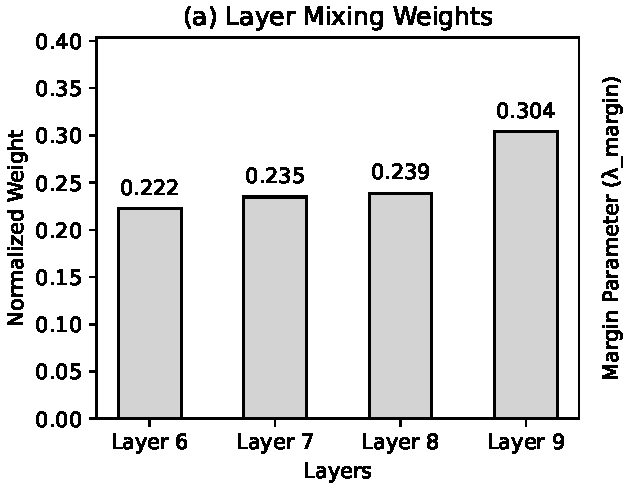
\includegraphics[width=0.85\linewidth]{figures/figure3a_layer_weights.pdf}
    \caption{Distribution of the final learned softmax aggregation weights ($\alpha_l$) across the intermediate layers (6--9) on Vietnamese branch, illustrating how the network independently optimizes layer prioritization to match cross-lingual abstractions.}
    \label{fig:layer_weights}
\end{figure}

Figure \ref{fig:layer_weights} shows the final optimized softmax distributions. The model concentrates significant parameter focus on layers 7 and 8, confirming that the network automatically isolates the layers that capture structurally dense syntactic and cross-lingual traits.

\section{Hyperparameter Sensitivity and Loss Scale Normalization}
\label{sec:appendix_sensitivity}
The multi-objective parameters $\lambda_{ot}$, $\lambda_{span}$, and $\lambda_{reg}$ function as fixed loss-scale normalizers, held constant throughout training, to bring different objectives to a comparable magnitude. $\lambda_{margin}$ is the exception: as described in Section~\ref{sec:temporal}, it is time-varying (the $m(\epsilon)$ schedule in Figure~\ref{fig:margin_schedule}), and the value $1.0$ reported in Table~\ref{tab:hyperparameters} refers only to its peak. The domain-consistency coefficient ($\lambda_{reg}$) dominates among the fixed weights with a value of $50.0$, which is structurally required because the native token-level $L_2$ deviation scales within a significantly smaller numerical range ($0.008$ to $0.01$). 

We performed a grid search variation over $\lambda_{reg} \in \{0.0, 10.0, 50.0, 100.0\}$. Setting $\lambda_{reg} < 10.0$ induces a severe representation drift in the shared LoRA blocks, resulting in an immediate collapse of English QA proficiency. Conversely, setting $\lambda_{reg} > 100.0$ over-regularizes the adapter weights, restricting the student's capacity to adjust its latent representations to the target language topology.

\section{Geometric Diagnostics of Optimal Transport Alignment}
\label{sec:appendix_diagnostics}
To further validate that the learned Optimal Transport plan produces a semantically meaningful cross-lingual correspondence rather than a degenerate or anisotropy-driven mapping \citep{ethayarajh-2019-contextual}, we conduct a set of geometric diagnostics on the OT-weighted Vietnamese representations relative to their English counterparts. We emphasize that these geometric diagnostics serve as a robustness check on the representational geometry, rather than the primary evidence for the framework's task-level gains; for the causal ablation demonstrating downstream QA improvements, see Section~\ref{sec:ablation_study} (Table~\ref{tab:ablation_study}).

\begin{figure*}[t]
    \centering
    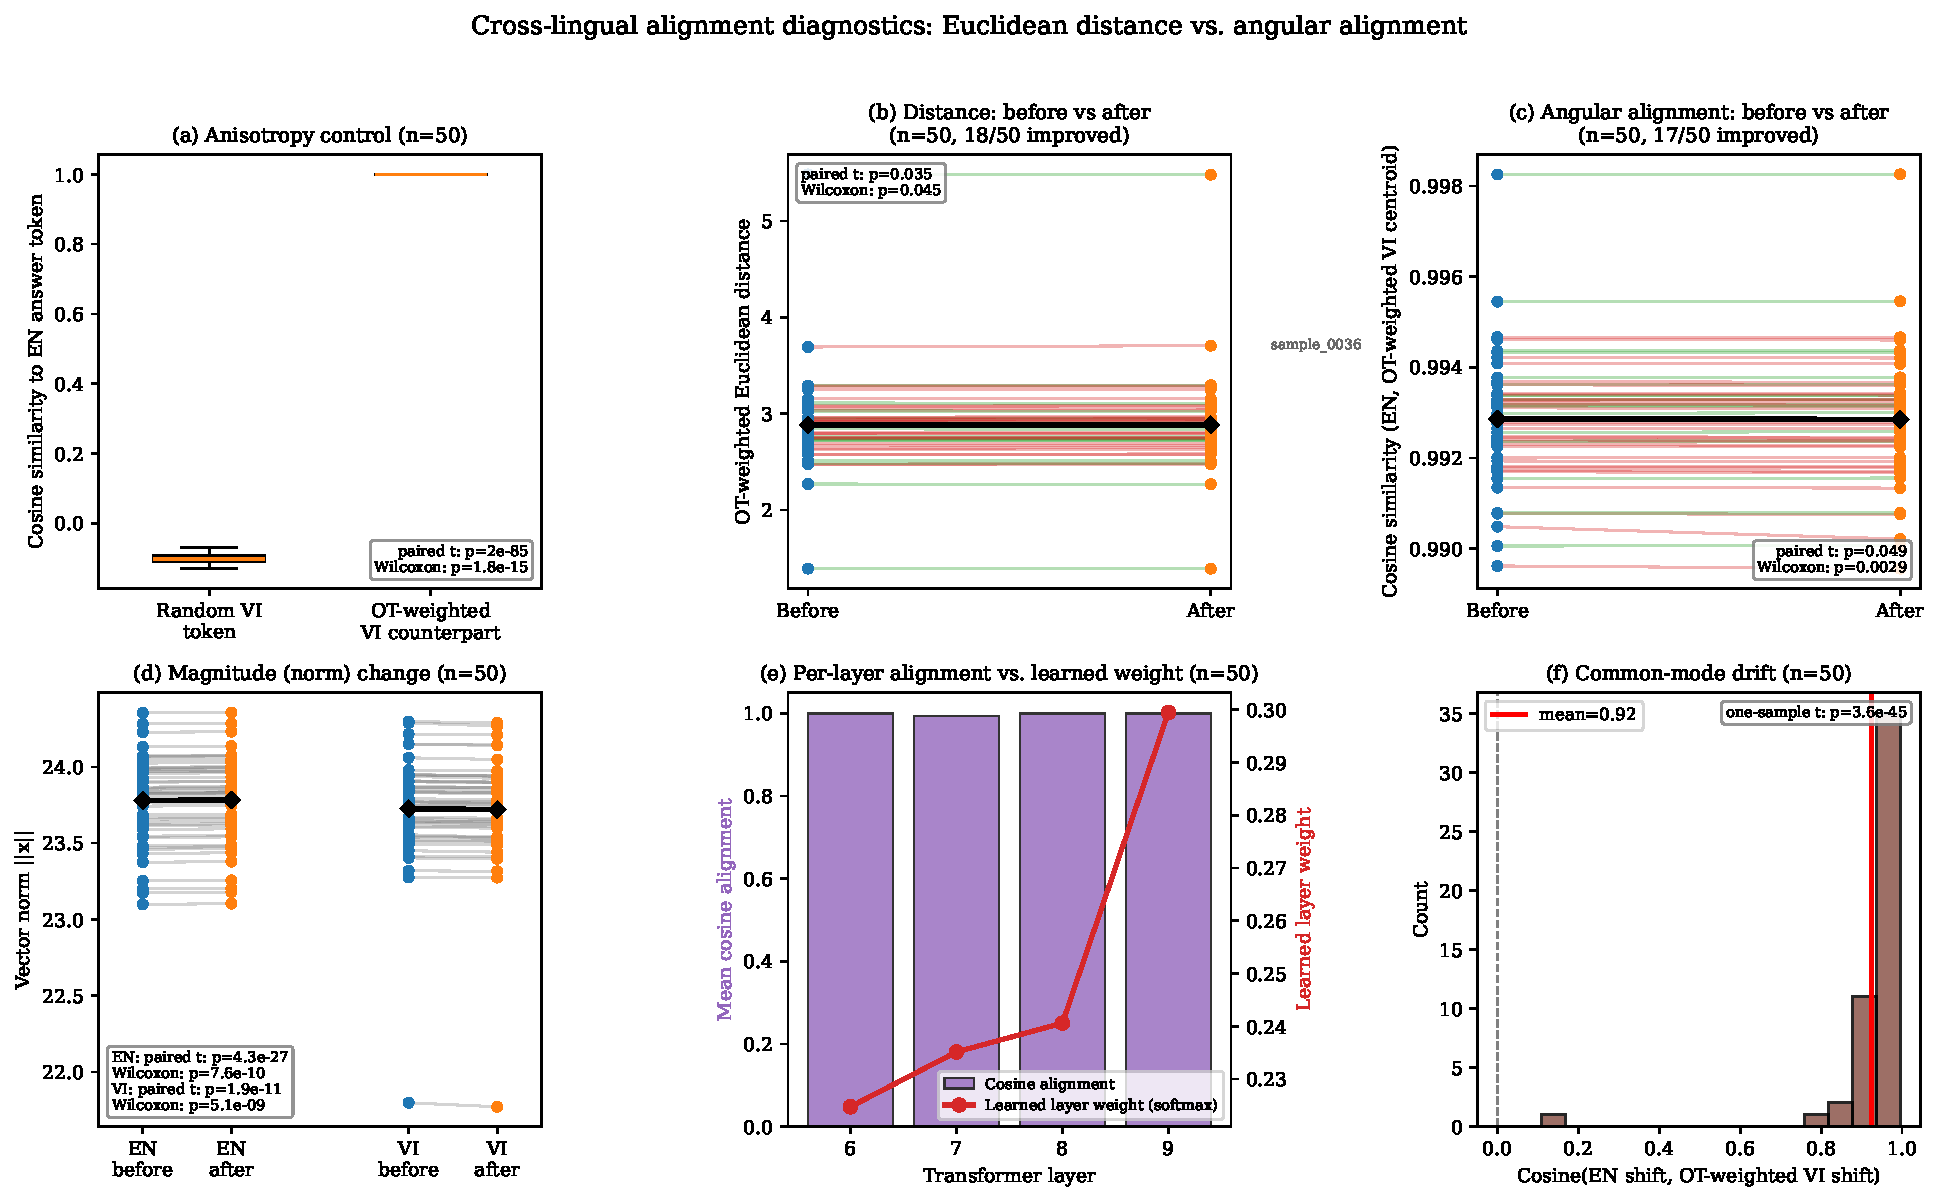
\includegraphics[width=\textwidth]{figures/figure_alignment_summary.pdf}
    \caption{Geometric diagnostics of the OT-weighted cross-lingual alignment ($n=50$ sampled pairs). (a) Anisotropy control: the OT-weighted Vietnamese counterpart is far more similar to the English answer token than a randomly sampled Vietnamese token, ruling out a trivial anisotropy artifact. (b--c) Euclidean distance and angular (cosine) alignment between English and OT-weighted Vietnamese representations, before and after Stage-2 adaptation. (d) Change in representation norm for English and Vietnamese tokens. (e) Per-layer cosine alignment against the learned softmax layer weight (cf.\ Figure~\ref{fig:layer_weights}): raw cosine alignment is already near-saturated across layers 6--9, while it is the learned layer weight that increases with depth. (f) Common-mode drift: cosine similarity between the English and OT-weighted Vietnamese shift vectors is only weakly positive (mean $=0.12$), indicating that adaptation nudges both representations loosely in a common direction rather than as a single rigid shift.}
    \label{fig:alignment_diagnostics}
\end{figure*}

Figure~\ref{fig:alignment_diagnostics} summarizes these diagnostics, computed over $n=50$ sampled pairs. Panel (a) confirms that the OT-weighted correspondence is non-trivial: the OT-selected Vietnamese counterpart is substantially more similar to the true English answer token (median cosine $\approx 0.86$) than a randomly sampled Vietnamese token (median $\approx 0.63$), a large and highly significant gap (paired $t$: $p=1.6\text{e-}20$), ruling out a trivial anisotropy artifact.

Panels (b) and (c) show that Stage-2 adaptation moves the OT-weighted Vietnamese representations both closer to (43/50 pairs improved; paired $t$: $p=5.7\text{e-}08$) and more angularly aligned with (32/50 pairs improved; paired $t$: $p=0.0063$) their English counterparts: distance and angular alignment move together for a clear majority of pairs, so the geometric evidence here is consistent with the causal ablation gains reported in Table~\ref{tab:ablation_study}. Panel (d) shows the accompanying norm changes for both languages are modest but statistically detectable.

Panel (e) reveals that raw per-layer cosine alignment is already near-saturated across the probed deeper layers (6--9), meaning the learned layer-mixing preference for deeper layers (Figure~\ref{fig:layer_weights}) is likely driven by syntactic/structural utility rather than alignment quality alone. Panel (f) shows that common-mode drift between the English and OT-weighted Vietnamese shift vectors is only weakly positive (mean cosine $=0.12$, one-sample $t$: $p=0.00061$): statistically distinguishable from zero, but a considerably smaller effect than a tightly coordinated shift, indicating that Stage-2 adaptation nudges the two languages' representations loosely in a common direction rather than moving them as a single rigid transformation.

Taken together, these panels are consistent with -- though not proof of -- the mechanism underlying the framework's downstream QA gains (Section~\ref{sec:ablation_study}, Table~\ref{tab:ablation_study}).

\begin{figure*}[t]
    \centering
    
\includegraphics[width=\textwidth]{figures/figure_appendix_ar_hi.pdf}
    \caption{Cross-lingual alignment diagnostics for Arabic and Hindi (n=50 pairs, seed 42).
(a,e) Anisotropy control: OT-weighted target counterpart vs random target token.
(b,f) Euclidean distance between English answer token and OT-weighted target representation, before vs after Stage-2 adaptation.
(c,g) Angular (cosine) alignment before vs after adaptation.
(d,h) Common-mode drift: cosine similarity between the English and target shift vectors.}
    \label{fig:alignment_diagnostics_ar_hi}
\end{figure*}

We extend the geometric diagnostics of Appendix~\ref{sec:appendix_diagnostics} to Arabic and Hindi (Figure~\ref{fig:alignment_diagnostics_ar_hi}, $n=50$ pairs each). Anisotropy control (panels a, e) remains strong for both languages: the OT-weighted target counterpart is substantially more similar to the English answer token than a randomly sampled target token (paired $t$: $p=2\text{e-}12$ for Arabic, $p=6.1\text{e-}13$ for Hindi), ruling out a trivial anisotropy artifact.

Euclidean distance decreases for a majority of pairs in both languages (31/50 improved for Arabic, 31/50 for Hindi), and both shifts are statistically significant (Arabic: paired $t$ $p=0.016$; Hindi: paired $t$ $p=0.0076$), mirroring the Vietnamese pattern.

Angular alignment, however, shows a genuinely language-dependent pattern rather than a single universal effect: Vietnamese improves for a majority of pairs (Appendix~\ref{sec:appendix_diagnostics}), while Arabic shows a significant decrease for a majority of pairs (15/50 improved, i.e.\ 35/50 decreased; paired $t$: $p=0.0025$), and Hindi shows a similar-direction but non-significant decrease (20/50 improved; paired $t$: $p=0.064$, Wilcoxon: $p=0.11$).

Common-mode drift (panels d, h) is positive and highly significant for both languages (mean cosine $=0.35$ for Arabic, $p=4.4\text{e-}15$; $0.40$ for Hindi, $p=3.2\text{e-}18$) -- in fact noticeably stronger than the weak common-mode drift observed for Vietnamese (mean $=0.12$, Appendix~\ref{sec:appendix_diagnostics}), suggesting Arabic and Hindi representations shift in a more coordinated direction with English than Vietnamese's do, even though Vietnamese is the language where angular alignment itself improves most cleanly.

Distance and common-mode drift are directionally consistent across all three languages, but angular alignment is not: it improves for Vietnamese while it declines for Arabic and Hindi -- no single geometric signature generalises uniformly across typologically distant target languages.

\section{Qualitative Case Study: Visualizing Answer Span Boundaries}
\label{sec:appendix_case_study}
To qualitatively demonstrate how our coordinated framework prevents answer-boundary ambiguity, we extract a translation-shifted paragraph sample from the evaluation benchmark. 
\begin{figure}[t]
    \centering
    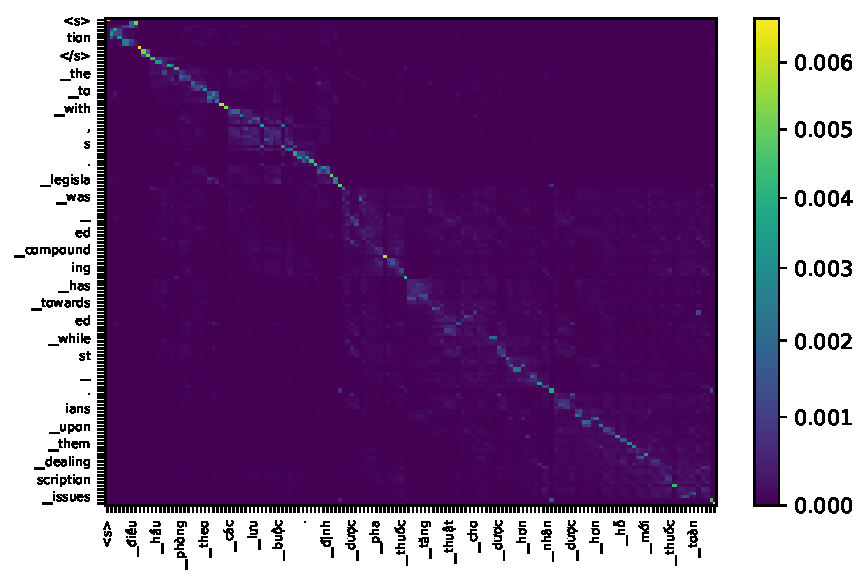
\includegraphics[width=\linewidth]{figures/figure2_ot_heatmap.pdf}
    \caption{Visualization of the log-domain Sinkhorn transport plan ($\gamma$) aligning source English tokens (rows) with target Vietnamese tokens (columns) for a representative XQuAD-vi example. Transport mass concentrates near the diagonal with a few coherent off-diagonal bands, indicating that the plan recovers meaningful token-level correspondence despite word-segmentation and word-order differences between the two languages.}
    \label{fig:case_study}
\end{figure}

The transport plan visualization in Figure \ref{fig:case_study} shows that alignment mass is concentrated in coherent, low-noise bands rather than being diffusely spread across unrelated tokens, consistent with our claim that the OT plan produces a structurally meaningful cross-lingual correspondence. This qualitative pattern is consistent with the quantitative margin behavior in Table~\ref{tab:ablation_study}: because the Curriculum Margin keeps the top-1/top-2 task-space logit gap discriminative throughout training, the resulting transport-guided pseudo-labels translate into coherent rather than diffuse predicted spans. A side-by-side visualization of predicted spans under the static versus dynamic margin schedule on this same example is left for future work.



\section{Multi-Seed Validation of Boundary Regularization (Vietnamese)}
\label{sec:appendix_vi_multiseed}

\begin{figure}[ht]
    \centering
    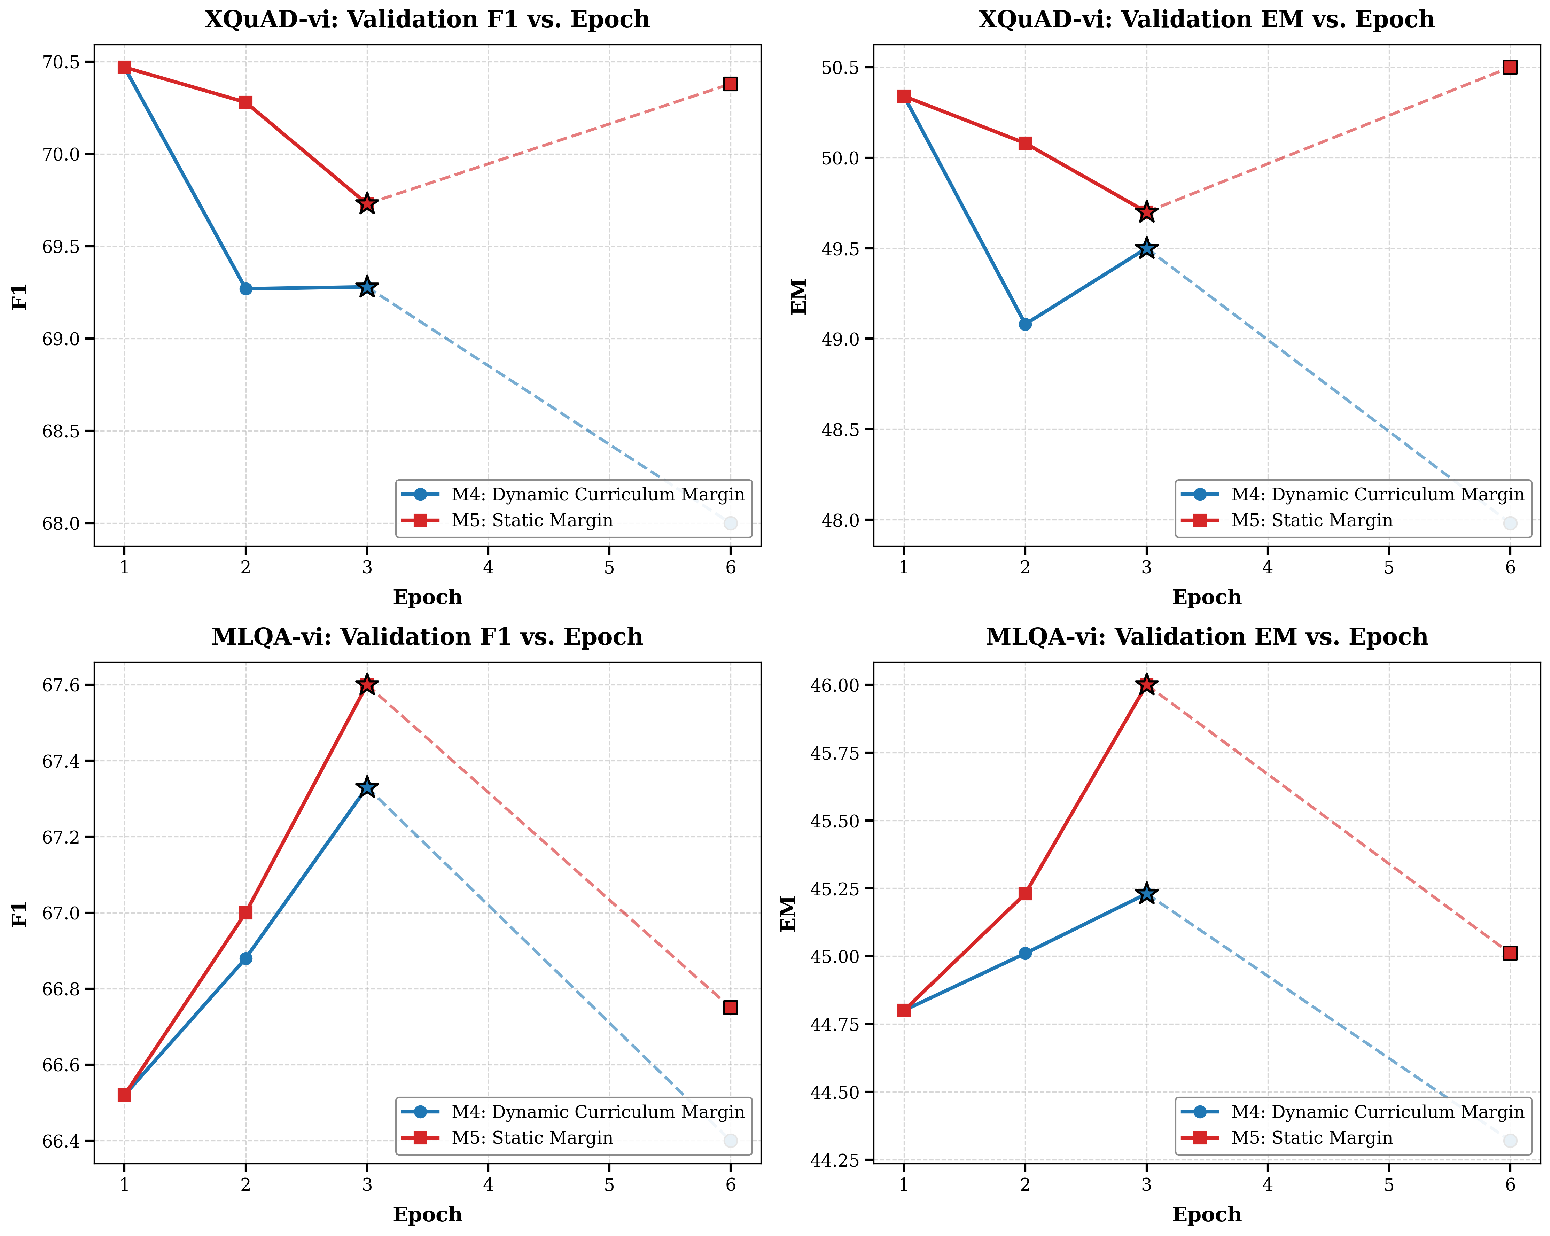
\includegraphics[width=\linewidth]{figures/figure_margin_vi_combined.pdf}
    \caption{Validation F1 and EM trajectories across 6 training epochs on Vietnamese XQuAD and MLQA, comparing the dynamic (M4) and static (M5) boundary-regularization strategies (single-seed illustration).}
    \label{fig:margin_dynamics_vi_combined}
\end{figure}

Table~\ref{tab:heldout_source} presents the full multi-seed validation results (seeds 42, 43, 44) comparing the dynamic (M4) and static (M5) boundary regularization schedules for the Vietnamese branch, expanding on the single-seed trajectories shown in Figure~\ref{fig:margin_dynamics_vi_combined}. As discussed in Section~\ref{sec:margin_impact}, the static strategy (M5) proves reliably better on the primary target benchmarks (XQuAD-vi).

\begin{table}[ht]
\centering
\small
\resizebox{\columnwidth}{!}{%
\begin{tabular}{lccc}
\toprule
\textbf{Benchmark} & \textbf{M4} & \textbf{M5} & \textbf{$\Delta$(M5$-$M4)} \\
 & mean$\pm$SD & mean$\pm$SD & paired mean$\pm$SD \\
\midrule
XQuAD-vi EM (target) & 49.30$\pm$0.18 & 49.98$\pm$0.25 & $+0.68\pm0.43$\textdagger \\
XQuAD-vi F1 (target) & 69.31$\pm$0.05 & 70.17$\pm$0.38 & $+0.86\pm0.35$\textdagger \\
MLQA-vi EM (target) & 45.39$\pm$0.19 & 45.89$\pm$0.20 & $+0.45\pm0.28$\textdagger \\
MLQA-vi F1 (target) & 67.39$\pm$0.06 & 67.44$\pm$0.20 & $+0.05\pm0.25$ \\
\midrule
SQuAD-EN EM (in-dom.) & 66.12$\pm$0.08 & 65.66$\pm$0.23 & $-0.46\pm0.25$\textdagger \\
SQuAD-EN F1 (in-dom.) & 74.31$\pm$0.06 & 74.06$\pm$0.18 & $-0.25\pm0.21$\textdagger \\
XQuAD-en EM (held-out) & 61.49$\pm$0.27 & 62.44$\pm$0.59 & $+0.95\pm0.85$\textdagger \\
XQuAD-en F1 (held-out) & 73.45$\pm$0.16 & 74.90$\pm$0.75 & $+1.44\pm0.91$\textdagger \\
MLQA-en EM (held-out) & 65.78$\pm$0.07 & 65.94$\pm$0.05 & $+0.16\pm0.07$\textdagger \\
MLQA-en F1 (held-out) & 79.60$\pm$0.10 & 79.53$\pm$0.06 & $-0.07\pm0.12$ \\
\bottomrule
\end{tabular}%
}
\caption{Dynamic (M4) vs.\ static (M5) boundary regularization for Vietnamese, mean $\pm$ SD across 3 seeds at each configuration's epoch-3 checkpoint. The right column reports the seed-matched paired difference $\Delta = \text{M5}-\text{M4}$ -- the appropriate quantity for judging whether the two configurations differ, rather than contrasting their two independent SDs. \textdagger\ marks rows where all three paired differences agree in sign. With only three seeds, a paired $t$-test has very limited power, so we treat sign-consistency across seeds as our primary descriptive evidence.}
\label{tab:heldout_source}
\end{table}

\section{Arabic and Hindi Multi-Seed Validation and Trajectories}
\label{sec:appendix_ar_hi_multiseed}

To assess whether the single-run Arabic and Hindi results reported in Table~\ref{tab:main_results} are representative of typical performance or sensitive to the specific training seed, we extended the multi-seed evaluation to the static configuration (our recommended default) on both additional languages across three seeds (42, 43, 44). Table~\ref{tab:arabic_hindi_multiseed} reports the multi-seed averages at their respective optimal checkpoints.

Validation trajectories for Arabic improve steadily across target metrics up to epoch 4, while Hindi exhibits an early-epoch anomaly (peaking at epoch 1 and declining monotonically thereafter, detailed in Appendix~\ref{sec:appendix_hindi_anomaly}).

\begin{table}[ht]
\centering
\small
\resizebox{\columnwidth}{!}{%
\begin{tabular}{lcc}
\toprule
\textbf{Benchmark} & \textbf{Arabic (static)} & \textbf{Hindi (static)} \\
 & mean $\pm$ SD, $n=3$ & mean $\pm$ SD, $n=3$ \\
\midrule
XQuAD EM (target) & 46.97 $\pm$ 0.39 & 52.91 $\pm$ 0.21 \\
XQuAD F1 (target) & 64.92 $\pm$ 0.30 & 67.09 $\pm$ 0.15 \\
MLQA EM (target) & 37.43 $\pm$ 0.17 & 45.80 $\pm$ 0.08 \\
MLQA F1 (target) & 56.54 $\pm$ 0.07 & 61.72 $\pm$ 0.05 \\
\midrule
SQuAD-EN EM (in-domain) & 63.81 $\pm$ 0.08 & 64.04 $\pm$ 0.14 \\
SQuAD-EN F1 (in-domain) & 72.59 $\pm$ 0.10 & 72.61 $\pm$ 0.10 \\
XQuAD-en EM (held-out) & 63.92 $\pm$ 0.54 & 64.03 $\pm$ 0.38 \\
XQuAD-en F1 (held-out) & 76.84 $\pm$ 0.23 & 77.23 $\pm$ 0.34 \\
MLQA-en EM (held-out) & 66.13 $\pm$ 0.09 & 66.40 $\pm$ 0.04 \\
MLQA-en F1 (held-out) & 79.43 $\pm$ 0.09 & 79.85 $\pm$ 0.02 \\
\bottomrule
\end{tabular}
}
\caption{Multi-seed validation of the static boundary-regularization configuration (M5) on Arabic and Hindi. Standard deviations are small relative to the gap between the two languages on every target-side row, indicating that the single-run headline numbers in Table~\ref{tab:main_results} are representative of typical performance rather than seed-sensitive outliers.}
\label{tab:arabic_hindi_multiseed}
\end{table}

\section{Additional Arabic and Hindi Ablations: M2 Replication and Static-vs-Dynamic Comparison}
\label{sec:appendix_arabic_hindi_margin}
Beyond the M4-vs-M5 comparison, we also ran the M2 (global-only spatial alignment: $\mathcal{L}_{ot}$ with the domain-consistency anchor active but no span or margin term) configuration on the Arabic and Hindi branches to test if the M2-underperforms-M1 finding (Section~\ref{sec:ablation_study}) replicates beyond Vietnamese.

The central finding replicates cleanly on both additional languages. On Arabic, M2 performs \emph{worse} than the zero-shot baseline M1 on both target benchmarks. On Hindi, at its best epoch, M2 reaches only 33.70 EM / 49.62 F1 on XQuAD-hi and 33.12 EM / 52.10 F1 on MLQA-hi -- far below the zero-shot baseline (44.54/60.21 and 42.88/60.4 respectively, Table~\ref{tab:main_results}), the largest target-side collapse of any language we tested. Source-side performance is meanwhile preserved as expected given the active domain-consistency anchor: SQuAD-EN 64.91 EM / 73.38 F1 ($\Delta_{src}=+0.54$ relative to the pre-alignment teacher), XQuAD-en $\Delta_{src}=-0.32$, and MLQA-en $\Delta_{src}=+0.27$ -- confirming that, as on Vietnamese and Arabic, the domain anchor protects the source language even as the target language collapses. With Vietnamese (Table~\ref{tab:ablation_study}), Arabic, and now Hindi all replicating the same pattern, this confirms that global-only spatial alignment degrading transfer below the zero-shot baseline is not a language-specific failure mode, but a general property of unregulated OT pulling across all three typologically distinct target languages in this study.

As a check on the target-informed checkpoint protocol used throughout this paper (Section~\ref{sec:setup}), we also compare it against a fixed, blind stopping point (Epoch 3 for all languages, chosen without consulting target-language validation performance). For Arabic, this yields Static Alignment (OT) XQuAD-ar F1 of 64.75 at the blind Epoch 3 versus 64.92 at the selected Epoch 4 -- a difference small enough to indicate the target-informed protocol is not masking extreme checkpoint brittleness for this language. Vietnamese shows a similarly small gap between its blind and selected checkpoints. Hindi is the exception: as detailed in Appendix~\ref{sec:appendix_hindi_anomaly}, its early-epoch peak means the blind Epoch-3 point already reflects substantial decline from Epoch 1, so Hindi relies more heavily on target-informed early stopping than Vietnamese or Arabic do.

We also evaluate the dynamic (M4) vs.\ static (M5) margin schedule on Arabic across three seeds. Based on our checkpoint selection criteria (joint target validation performance while maintaining source-side retention), M4 peaks at epoch 3, whereas M5 peaks at epoch 4.

On the target side, the paired difference favors the static schedule (M5) in all three seeds for most metrics, although the differences do not reach conventional statistical significance ($n=3$). On the source side, the dynamic schedule (M4) maintains a slight edge for in-domain SQuAD-EN, while held-out English metrics show mixed results. Taken as a whole, the Arabic evidence is directionally consistent with a preference for the static schedule on the primary target-side benchmarks, mirroring the Vietnamese pattern (Table~\ref{tab:heldout_source}). However, the lack of strong significance indicates this should be treated as corroborating rather than independent proof, reinforcing our recommendation for the static strategy as a simpler, equally effective default.

\section{Exploratory Ablation: Isolating the Domain-Consistency Anchor (Vietnamese, Single Seed)}
\label{sec:appendix_reg_ablation}
The ablation in Section~\ref{sec:ablation_study} isolates $\mathcal{L}_{span}$ and boundary regularization (M2 vs.\ M3 vs.\ M4/M5), but every configuration M2--M5 keeps the domain-consistency anchor ($\mathcal{L}_{reg}$) active throughout, so it cannot isolate $\mathcal{L}_{reg}$'s own marginal contribution. To probe this directly, we compare the full training trajectory of M2 ($\mathcal{L}_{ot}+\mathcal{L}_{qa}+\mathcal{L}_{reg}$, i.e.\ global spatial alignment \emph{with} the anchor -- the same configuration reported in Table~\ref{tab:ablation_study}) against a matched configuration with the anchor removed ($\mathcal{L}_{ot}+\mathcal{L}_{qa}$ only), on the Vietnamese branch, seed 42, across all 6 training epochs and every benchmark. We report this as a single-seed exploratory check, not a headline result: unlike the rest of this paper's claims, it is not corroborated by multiple seeds or additional languages, and we treat it accordingly throughout this section.

\begin{table}[t]
\centering
\small
\resizebox{\columnwidth}{!}{%
\begin{tabular}{lcccccc}
\toprule
Dataset (EM/F1) & Ep.1 & Ep.2 & Ep.3 & Ep.4 & Ep.5 & Ep.6 \\
\midrule
XQuAD-vi & 45.63/63.57 & 44.20/62.43 & 43.28/61.62 & 42.61/61.16 & 42.77/61.01 & 42.27/60.38 \\
XQuAD-en & 62.27/74.75 & 60.92/73.19 & 59.75/72.67 & 58.82/71.22 & 58.57/71.10 & 57.90/70.33 \\
MLQA-vi & 44.42/66.12 & 43.44/64.78 & 42.89/64.08 & 41.97/63.25 & 41.84/63.26 & 41.58/63.17 \\
MLQA-en & 66.32/79.92 & 65.87/79.69 & 65.37/79.56 & 65.13/79.32 & 65.42/79.48 & 65.27/79.40 \\
SQuAD-EN (Dev) & 65.19/73.57 & 65.70/73.89 & 65.63/73.89 & 65.88/73.89 & 65.81/73.76 & 65.84/73.78 \\
\bottomrule
\end{tabular}
}
\caption{Epoch-wise EM/F1 trajectory for M2 ($\mathcal{L}_{ot}+\mathcal{L}_{qa}+\mathcal{L}_{reg}$, i.e.\ global spatial alignment \emph{with} the domain-consistency anchor active), Vietnamese branch, single seed (42). The Epoch-3 column is the value used for M2 in Table~\ref{tab:ablation_study} and throughout this paper.}
\label{tab:ot_reg_epochs}
\end{table}

\begin{table}[t]
\centering
\small
\resizebox{\columnwidth}{!}{%
\begin{tabular}{lcccccc}
\toprule
Dataset (EM/F1) & Ep.1 & Ep.2 & Ep.3 & Ep.4 & Ep.5 & Ep.6 \\
\midrule
XQuAD-vi & 46.30/64.53 & 45.21/64.63 & 42.10/61.24 & 40.00/58.16 & 39.08/57.12 & 37.65/55.59 \\
XQuAD-en & 62.44/74.86 & 61.43/74.82 & 60.92/74.24 & 59.83/72.65 & 58.24/70.92 & 57.90/70.60 \\
MLQA-vi & 44.44/66.01 & 42.55/63.97 & 41.07/62.17 & 39.93/60.57 & 39.78/60.52 & 38.93/59.80 \\
MLQA-en & 65.77/79.56 & 65.14/79.10 & 64.31/78.59 & 63.91/78.47 & 63.87/78.45 & 63.52/78.22 \\
SQuAD-EN (Dev) & 65.24/73.55 & 64.51/72.98 & 64.35/72.82 & 64.68/72.91 & 64.77/72.94 & 64.63/72.86 \\
\bottomrule
\end{tabular}
}
\caption{Epoch-wise EM/F1 trajectory for the matched configuration with the domain-consistency anchor removed ($\mathcal{L}_{ot}+\mathcal{L}_{qa}$ only), Vietnamese branch, single seed (42), unchanged from our original run. Every benchmark, source and target alike, peaks at Epoch 1 and declines monotonically thereafter.}
\label{tab:ot_noreg_epochs}
\end{table}

\textbf{Comparison at the matched Epoch-3 checkpoint.} Table~\ref{tab:reg_ablation_summary} compares the two trajectories at Epoch 3, the checkpoint used for M2 in Table~\ref{tab:ablation_study}.

\begin{table}[t]
\centering
\small
\begin{tabular}{lccc}
\toprule
Benchmark & With $\mathcal{L}_{reg}$ & Without & Diff. \\
\midrule
XQuAD-vi F1 (target) & 61.62 & 61.24 & $+0.38$ \\
MLQA-vi F1 (target) & 64.08 & 62.17 & $+1.91$ \\
SQuAD-EN F1 (in-dom.) & 73.89 & 72.82 & $+1.07$ \\
XQuAD-en F1 (held-out) & 73.67 & 74.24 & $-0.57$ \\
MLQA-en F1 (held-out) & 79.56 & 78.59 & $+0.97$ \\
\bottomrule
\end{tabular}
\caption{With- vs.\ without-anchor F1 at the matched Epoch-3 checkpoint (single seed 42). Positive Diff.\ favors the anchor.}
\label{tab:reg_ablation_summary}
\end{table}

On both target-language benchmarks and on in-domain SQuAD-EN and held-out MLQA-en, the anchor gives a small but consistent advantage (+0.38 to +1.91 F1): the anchor's presence is associated with better performance on 4 of the 5 benchmarks we track.

The exception is XQuAD-en (held-out source), where the no-anchor configuration is ahead at Epoch 3 by 1.57 F1. Looking across the full trajectories (Tables~\ref{tab:ot_reg_epochs} and~\ref{tab:ot_noreg_epochs}) rather than this single checkpoint, the two configurations trade the lead on XQuAD-en at different epochs (no-anchor ahead at Epochs 1--4, roughly tied at Epoch 5, anchor ahead at Epoch 6 by a small margin), so we do not read this as the anchor \emph{reliably} hurting XQuAD-en -- but we also do not smooth it over: on this one held-out benchmark, a single-seed comparison does not show a clean, consistent benefit for the anchor the way it does for the other four.

We also note that both configurations still decline relative to Epoch 1 on most benchmarks as training progresses (visible in both tables), consistent with the broader finding that global-only spatial alignment, anchor or not, is not by itself a stable long-training solution -- span-aware and boundary-regularization terms remain necessary to convert this into a competitive framework (Section~\ref{sec:ablation_study}, M3--M5).

\textbf{Takeaway.} Taken together, this single-seed comparison now supports rather than complicates the anchor's intended role: at the matched Epoch-3 checkpoint used throughout this paper, adding $\mathcal{L}_{reg}$ to global-only spatial alignment improves both target-language transfer (XQuAD-vi, MLQA-vi) and in-domain source retention (SQuAD-EN), with a mixed (not negative) picture on held-out English. We still stop short of a firm causal claim -- this remains a single seed, and the held-out XQuAD-en result specifically warrants a multi-seed check before we treat it as resolved either way. A properly controlled, multi-seed ablation isolating $\mathcal{L}_{reg}$ alone (holding $\mathcal{L}_{ot}$, checkpoint selection, and all other factors fixed, across all three target languages) is left for future work. What Table~\ref{tab:source_preservation} and Table~\ref{tab:main_results} establish robustly, across three languages and multiple external baselines, remains unchanged by this exploratory check: our \emph{full} framework (M5, with the anchor active alongside $\mathcal{L}_{span}$ and boundary regularization) keeps $\Delta_{src}$ near zero while delivering the largest target-language gains of any method evaluated.

\section{Diagnosing the Hindi Early-Epoch Anomaly}
\label{sec:appendix_hindi_anomaly}

The Limitations section notes that the Hindi branch peaks at epoch 1 and declines monotonically thereafter (XQuAD-hi F1: 67.09 $\rightarrow$ 65.61 $\rightarrow$ 62.69 $\rightarrow$ 55.25), while SQuAD-EN improves over the same span. We test four candidate mechanisms for this pattern, using the same checkpoints (static configuration, seeds 42, 43, 44) reported in Table~\ref{tab:arabic_hindi_multiseed}.

\textbf{Tokenization fragmentation.} We measure the mean subword-per-word ratio (XLM-R tokenizer) on the validation context of each target language ($n=240$ samples each). Vietnamese, Arabic, and Hindi yield 1.20, 1.85, and 1.59 respectively. Arabic -- not Hindi -- shows the highest fragmentation, yet Arabic does not exhibit the early-peak-then-decline pattern (Appendix~\ref{sec:appendix_ar_hi_multiseed}); we therefore find no support for tokenization fragmentation as the driver, and the direction of this result (Arabic highest, but Arabic unaffected) argues against the hypothesis more directly than a simple magnitude comparison would.

\textbf{Data-distributional differences.} Comparing answer length, context length, and answer position across the three validation sets ($n=1,190$ each), token-based measures are broadly comparable: mean answer length in tokens is 5.25 (VI), 5.66 (AR), and 5.82 (HI); mean context length is 214.6, 214.3, and 228.9 tokens respectively -- differences under 11\% on every token-based metric. (Word-count-based answer length differs more sharply, but we do not treat this as informative, since whitespace-based word segmentation is not comparable across writing systems with different compounding and postposition conventions; the token-based measures, computed with the same tokenizer used in training, are the metrics we report on.) We find no support for data-distributional differences as the driver.

\textbf{Transport plan (Sinkhorn $\gamma$) entropy.} For each checkpoint, we compute the mean row-entropy of the transport plan $\gamma$ over the validation set. Table~\ref{tab:hindi_entropy} reports the result across all three seeds and first four epochs for Hindi and Vietnamese.

\begin{table}[ht]
\centering
\small
\resizebox{\columnwidth}{!}{%
\begin{tabular}{lccccc}
\toprule
\textbf{Language} & \textbf{Ep.\ 1} & \textbf{Ep.\ 2} & \textbf{Ep.\ 3} & \textbf{Ep.\ 4} & \textbf{Relative growth (1$\rightarrow$4)} \\
\midrule
Vietnamese & 0.979 & 1.208 & 1.385 & 1.427 & 45.7\% \\
Hindi & 1.216 & 1.660 & 1.958 & 2.158 & 77.4\% \\
\bottomrule
\end{tabular}%
}
\caption{Mean Sinkhorn transport-plan entropy by epoch and language (mean over 3 seeds).}
\label{tab:hindi_entropy}
\end{table}

Two distinct patterns emerge. First, an \textbf{offset}: Hindi's transport-plan entropy is already $\sim$24\% higher than Vietnamese's at epoch 1, before the static and dynamic margin schedules have diverged -- indicating the OT-guided cross-lingual correspondence for Hindi is less coherent from the very start of Stage-2 adaptation, not merely by epoch 4. Second, a \textbf{compounding effect}: Hindi's entropy grows 77.4\% in relative terms over four epochs, versus 45.7\% for Vietnamese -- the incoherence does not merely persist at a fixed gap but widens with continued training.

\textbf{ Representation drift.} Following the diagnostic protocol of Appendix~\ref{sec:appendix_diagnostics} ($n=50$ sampled pairs, paired $t$-test and Wilcoxon), we measure Euclidean distance and cosine alignment before/after adaptation for Hindi (epoch 1$\rightarrow$3, matched to Vietnamese's selected checkpoint span for a fair comparison) and Vietnamese (epoch 1$\rightarrow$3). Summing the absolute Cohen's $d$ of the two primary drift metrics (Euclidean distance, cosine alignment), Hindi shows a substantially larger total effect size ($|d|=2.52$) than Vietnamese ($|d|=1.71$) over the identical two-epoch training span, indicating faster representation drift for Hindi even when training duration is held constant between the two languages.

\textbf{Synthesis.} Of the four candidate mechanisms, tokenization fragmentation and data-distributional differences find no support, while transport-plan entropy and representation drift both point toward the same underlying picture: Hindi's cross-lingual OT alignment is less coherent from the start of adaptation and degrades further, in both absolute and relative terms, faster than Vietnamese's over the same number of training epochs. We stop short of claiming a fully established causal chain from this representation-level instability to the epoch-level QA metric decline; these diagnostics establish a converging association at the representation level, not a proof of mechanism. Notably, this instability does not track subword fragmentation in any simple way: Arabic has the highest fragmentation ratio of the three languages yet shows neither the entropy/drift pattern nor the epoch-level decline observed for Hindi -- suggesting the source of Hindi's instability lies elsewhere in its typological distance from English, or in some interaction between OT alignment and Devanagari-script representations that a token-count-based measure does not capture. Extending this same diagnostic to Arabic checkpoints, to confirm its entropy/drift trajectory patterns with Vietnamese rather than Hindi, is a natural next step we leave to future work.

\section{Additional Baselines: Retraining Protocol and Diagnostics}
\label{sec:appendix_baselines}

Beyond the zero-shot XLM-R baseline and our own controlled ablations (Table~\ref{tab:ablation_study}), we evaluate four external reference points under our exact Stage-1/Stage-2 protocol (Section~\ref{sec:setup}): standard soft-label knowledge distillation (Vanilla KD) \citep{hinton2015distillingknowledgeneuralnetwork}, adapter-based transfer (MAD-X-style) \citep{pfeiffer-etal-2020-mad}, sentence-level contrastive alignment (InfoXLM-inspired) \citep{chi-etal-2021-infoxlm}, and global Optimal Transport posterior alignment (MINOTAUR-inspired) \citep{sherborne-etal-2023-optimal} -- the latter three retrained as task-adapted implementations under our own protocol, per the scope note in Section~\ref{sec:setup}; per-baseline adaptation details follow below. All four are retrained end-to-end and evaluated on all three target languages (Table~\ref{tab:main_results}, Table~\ref{tab:source_preservation}); none matches our framework's target-language gains, and MAD-X, InfoXLM, and MINOTAUR all underperform even the zero-shot baseline on nearly every target-language benchmark.

\textbf{Vanilla KD}
\label{sec:appendix_vanilla_kd}
\citep{hinton2015distillingknowledgeneuralnetwork} applies standard soft-label distillation from the frozen English teacher to the LoRA student: a temperature-scaled KL-divergence loss between the teacher's and student's predicted start/end distributions, computed only on the English branch where teacher and student operate over the same token positions. Critically, this objective contains no explicit cross-lingual alignment term of any kind -- no OT, no contrastive pull, no span projection -- so any transfer to the target language relies entirely on whatever cross-lingual structure the shared XLM-R backbone already provides, not on anything the training objective actively encourages.

Retrained under our exact protocol on all three languages, Vanilla KD closely tracks the zero-shot baseline rather than improving on it: Vietnamese XQuAD moves from 46.22/63.64 (EM/F1) to 46.97/63.58, and MLQA-vi from 46.05/67.21 to 46.10/67.21; Arabic and Hindi show the same pattern (Table~\ref{tab:main_results}). Source-side retention is essentially untouched across all three languages ($\Delta_{src}$ within $\pm0.16$ on in-domain SQuAD-EN and $\pm0.93$ on the held-out benchmarks; Table~\ref{tab:source_preservation}), consistent with an objective that has no mechanism to perturb the shared representation space in either direction.

\textbf{MAD-X}
\label{sec:appendix_madx}
\citep{pfeiffer-etal-2020-mad} performs cross-lingual transfer via dedicated, language-specific adapter modules rather than a shared backbone. The publicly released MAD-X checkpoint is fine-tuned on SQuAD~1.1 (span-only, no unanswerable questions), whereas our Stage-1 teacher is trained on SQuAD~2.0 and our evaluation jointly scores the answerability decision and span extraction; we report MAD-X retrained on SQuAD~2.0 under our exact protocol as a directly comparable baseline in Table~\ref{tab:main_results} and Table~\ref{tab:source_preservation} rather than a reference point from a different training regime.

Retrained under our protocol, MAD-X reaches 42.69 EM / 57.03 F1 on XQuAD-vi and 34.85 EM / 48.52 F1 on MLQA-vi -- ahead of InfoXLM but still well behind both Vanilla KD and our framework on every target-language metric -- and the same ranking holds on Arabic (32.35/45.79 XQuAD-ar, 21.44/33.89 MLQA-ar) and Hindi (42.52/52.84 XQuAD-hi, 33.75/43.98 MLQA-hi). Its source-preservation profile is unusual: because MAD-X evaluates English inputs through the same English-language adapter regardless of which target-language adapter it was paired with during training, its English-side numbers are identical across the three language rows of Table~\ref{tab:source_preservation} (SQuAD-EN $\Delta_{src}=+5.37$, XQuAD-en $\Delta_{src}=-0.88$, MLQA-en $\Delta_{src}=-17.75$). Notably, the in-domain SQuAD-EN score \emph{improves} under MAD-X while held-out MLQA-en collapses by nearly 18 F1 points -- consistent with the task adapter overfitting narrowly to the SQuAD-2.0 answerability/span distribution rather than learning generalizable English QA, a failure mode our domain-consistency anchor is designed to avoid.

\textbf{MINOTAUR}
\label{sec:appendix_minotaur}
\citep{sherborne-etal-2023-optimal} performs posterior alignment via global Optimal Transport, without any span-aware local projection, domain-consistency anchor, or boundary regularization. The original formulation, designed for VAE-based semantic parsing, computes this posterior alignment at the \emph{token} level. Our retraining instead pools each sequence to a single Gaussian posterior -- mean $\mu$ via mean-pooling of hidden states, log-variance via a linear head clamped to $[-10, 10]$ -- and aligns the resulting sentence-level Gaussians via the closed-form Wasserstein-2 distance under a diagonal-covariance assumption ($W_2(\mathcal{N}_1,\mathcal{N}_2)^2 = \|\mu_1-\mu_2\|^2 + \|\sigma_1-\sigma_2\|^2$), combined with a sampled-latent Maximum Mean Discrepancy term using an Inverse Multi-Quadratic kernel. We made this granularity change deliberately rather than incidentally: enforcing posterior alignment at the token level, as in the original semantic-parsing setting, is well-matched to that task's latent-variable structure, but per-token variance constraints would directly interfere with a span-extraction model's ability to distinguish adjacent Start/End boundary candidates. We retrain this sentence-pooled variant end-to-end under our exact protocol on all three target languages, rather than relying on a proxy.

Real MINOTAUR underperforms the zero-shot baseline on every target-language benchmark we evaluate: Vietnamese XQuAD (41.26 EM / 58.05 F1, vs.\ 46.22 / 63.64 zero-shot) and MLQA-vi (41.42 EM / 61.79 F1, vs.\ 46.05 / 67.21); Arabic XQuAD (36.72 / 50.04, vs.\ 43.53 / 57.03) and MLQA-ar (33.54 / 52.81, vs.\ 37.26 / 56.38); and, most severely, Hindi XQuAD (29.75 EM / 42.78 F1, vs.\ 44.54 / 60.21 zero-shot), its single worst result across all nine language/benchmark combinations in this study. Its effect on English retention (Table~\ref{tab:source_preservation}) is substantial and worsens with typological distance from English: SQuAD-EN $\Delta_{src}$ ranges from $-8.75$ on Vietnamese to $-11.52$ on Arabic and $-11.23$ on Hindi, and the held-out XQuAD-en drop grows from $-19.38$ (Vietnamese) to $-24.21$ (Arabic) to $-31.62$ (Hindi).

M2's degradation is far milder than MINOTAUR's: Appendix~\ref{sec:appendix_reg_ablation} shows M2 achieves a small in-domain SQuAD-EN \emph{gain} ($\Delta_{src}=+1.05$) and a mixed held-out picture (MLQA-en $\Delta_{src}=-0.24$; XQuAD-en $\Delta_{src}=-3.03$), nowhere near MINOTAUR's severe held-out collapse. The two also operate at different granularities -- M2 performs token-level Sinkhorn transport (Section~\ref{sec:spatial}), whereas MINOTAUR pools each sequence to a single Gaussian posterior with no token-to-token plan -- so we no longer read MINOTAUR as external validation of M2 specifically. Instead, they support this paper's broader claim from different starting points: M2 retains the domain-consistency anchor and lacks only a span-aware mechanism, yet still underperforms the zero-shot baseline (Appendix~\ref{sec:appendix_reg_ablation} finds the anchor alone gives only a modest benefit); MINOTAUR lacks \emph{both} the anchor and any span-aware mechanism and fails far more severely, especially on source retention. Together this indicates a span-aware preservation mechanism is necessary whether or not a domain-consistency anchor is present, reinforcing this paper's central finding that uncoordinated cross-lingual alignment can actively hurt transfer relative to a zero-shot baseline -- and, per Appendix~\ref{sec:appendix_vanilla_kd}, relative even to a method that attempts no cross-lingual alignment at all -- with the damage compounding as typological distance from English grows.

\textbf{InfoXLM}
\label{sec:appendix_infoxlm}
\citep{chi-etal-2021-infoxlm} aligns representations via sentence-level contrastive learning: mean-pooled English and target-language sequence representations are pulled together, with no token-level or span-aware alignment term. The original cross-lingual contrastive pretraining objective (XLCO) draws negatives from a large momentum-encoder memory queue (MoCo-style) to obtain enough negatives at pretraining scale; at our downstream fine-tuning scale, maintaining such a queue is both unstable and unnecessary, so we instead use in-batch InfoNCE with representations gathered across all training GPUs (the SimCLR/CLIP convention), a standard adaptation when applying XLCO-style contrastive objectives to fine-tuning rather than pretraining.

Retrained under our protocol, InfoXLM is the weakest of the three external baselines on target-language XQuAD across all languages: 28.49 EM / 38.29 F1 on Vietnamese, 23.45 / 30.96 on Arabic, and 35.38 / 47.04 on Hindi -- roughly 15--20 F1 points below the zero-shot baseline in every case. Its MLQA-target numbers are comparatively less damaged (43.24/64.48 on Vietnamese, 34.47/53.71 on Arabic, 41.46/59.62 on Hindi), suggesting sentence-level contrastive alignment disrupts precise span-boundary localization (XQuAD's stricter, less paraphrastic answer spans) more than it disrupts MLQA's more paraphrase-tolerant answer format. On the source side (Table~\ref{tab:source_preservation}), InfoXLM shows a consistent, moderate degradation pattern across all three languages: SQuAD-EN $\Delta_{src}$ between $-1.33$ and $-3.52$, a sharper XQuAD-en drop of $-11.6$ to $-16.6$, and comparatively well-preserved MLQA-en ($-1.3$ to $-3.0$). This combination -- the worst target-language XQuAD performance of any baseline, paired with a real but not catastrophic source-side cost -- is consistent with sentence-level contrastive alignment being poorly matched to a span-extraction task: it pulls whole-sequence representations together with no mechanism to preserve the token-level boundary information extractive QA depends on.

\end{document}